\documentclass[twoside]{book}

% Packages required by doxygen
\usepackage{calc}
\usepackage{doxygen}
\usepackage{graphicx}
\usepackage[utf8]{inputenc}
\usepackage{makeidx}
\usepackage{multicol}
\usepackage{multirow}
\usepackage{textcomp}
\usepackage[table]{xcolor}

% Font selection
\usepackage[T1]{fontenc}
\usepackage{mathptmx}
\usepackage[scaled=.90]{helvet}
\usepackage{courier}
\usepackage{amssymb}
\usepackage{sectsty}
\renewcommand{\familydefault}{\sfdefault}
\allsectionsfont{%
  \fontseries{bc}\selectfont%
  \color{darkgray}%
}
\renewcommand{\DoxyLabelFont}{%
  \fontseries{bc}\selectfont%
  \color{darkgray}%
}

% Page & text layout
\usepackage{geometry}
\geometry{%
  a4paper,%
  top=2.5cm,%
  bottom=2.5cm,%
  left=2.5cm,%
  right=2.5cm%
}
\tolerance=750
\hfuzz=15pt
\hbadness=750
\setlength{\emergencystretch}{15pt}
\setlength{\parindent}{0cm}
\setlength{\parskip}{0.2cm}
\makeatletter
\renewcommand{\paragraph}{%
  \@startsection{paragraph}{4}{0ex}{-1.0ex}{1.0ex}{%
    \normalfont\normalsize\bfseries\SS@parafont%
  }%
}
\renewcommand{\subparagraph}{%
  \@startsection{subparagraph}{5}{0ex}{-1.0ex}{1.0ex}{%
    \normalfont\normalsize\bfseries\SS@subparafont%
  }%
}
\makeatother

% Headers & footers
\usepackage{fancyhdr}
\pagestyle{fancyplain}
\fancyhead[LE]{\fancyplain{}{\bfseries\thepage}}
\fancyhead[CE]{\fancyplain{}{}}
\fancyhead[RE]{\fancyplain{}{\bfseries\leftmark}}
\fancyhead[LO]{\fancyplain{}{\bfseries\rightmark}}
\fancyhead[CO]{\fancyplain{}{}}
\fancyhead[RO]{\fancyplain{}{\bfseries\thepage}}
\fancyfoot[LE]{\fancyplain{}{}}
\fancyfoot[CE]{\fancyplain{}{}}
\fancyfoot[RE]{\fancyplain{}{\bfseries\scriptsize Generated on Sun Dec 8 2013 19\-:44\-:56 for My Project by Doxygen }}
\fancyfoot[LO]{\fancyplain{}{\bfseries\scriptsize Generated on Sun Dec 8 2013 19\-:44\-:56 for My Project by Doxygen }}
\fancyfoot[CO]{\fancyplain{}{}}
\fancyfoot[RO]{\fancyplain{}{}}
\renewcommand{\footrulewidth}{0.4pt}
\renewcommand{\chaptermark}[1]{%
  \markboth{#1}{}%
}
\renewcommand{\sectionmark}[1]{%
  \markright{\thesection\ #1}%
}

% Indices & bibliography
\usepackage{natbib}
\usepackage[titles]{tocloft}
\setcounter{tocdepth}{3}
\setcounter{secnumdepth}{5}
\makeindex

% Hyperlinks (required, but should be loaded last)
\usepackage{ifpdf}
\ifpdf
  \usepackage[pdftex,pagebackref=true]{hyperref}
\else
  \usepackage[ps2pdf,pagebackref=true]{hyperref}
\fi
\hypersetup{%
  colorlinks=true,%
  linkcolor=blue,%
  citecolor=blue,%
  unicode%
}

% Custom commands
\newcommand{\clearemptydoublepage}{%
  \newpage{\pagestyle{empty}\cleardoublepage}%
}


%===== C O N T E N T S =====

\begin{document}

% Titlepage & ToC
\hypersetup{pageanchor=false}
\pagenumbering{roman}
\begin{titlepage}
\vspace*{7cm}
\begin{center}%
{\Large My Project }\\
\vspace*{1cm}
{\large Generated by Doxygen 1.8.5}\\
\vspace*{0.5cm}
{\small Sun Dec 8 2013 19:44:56}\\
\end{center}
\end{titlepage}
\clearemptydoublepage
\tableofcontents
\clearemptydoublepage
\pagenumbering{arabic}
\hypersetup{pageanchor=true}

%--- Begin generated contents ---
\chapter{Hierarchical Index}
\section{Class Hierarchy}
This inheritance list is sorted roughly, but not completely, alphabetically\-:\begin{DoxyCompactList}
\item \contentsline{section}{Factory}{\pageref{classFactory}}{}
\item \contentsline{section}{T\-C\-P\-Server\-:\-:Hook}{\pageref{structTCPServer_1_1Hook}}{}
\item \contentsline{section}{intrusive\-\_\-ptr$<$ T $>$}{\pageref{classintrusive__ptr}}{}
\item list\begin{DoxyCompactList}
\item \contentsline{section}{Groupe}{\pageref{classGroupe}}{}
\end{DoxyCompactList}
\item \contentsline{section}{Pointable}{\pageref{classPointable}}{}
\begin{DoxyCompactList}
\item \contentsline{section}{Groupe}{\pageref{classGroupe}}{}
\item \contentsline{section}{Source}{\pageref{classSource}}{}
\begin{DoxyCompactList}
\item \contentsline{section}{Photo}{\pageref{classPhoto}}{}
\item \contentsline{section}{Video}{\pageref{classVideo}}{}
\begin{DoxyCompactList}
\item \contentsline{section}{Film}{\pageref{classFilm}}{}
\end{DoxyCompactList}
\end{DoxyCompactList}
\end{DoxyCompactList}
\item \contentsline{section}{Server\-Socket}{\pageref{classServerSocket}}{}
\item \contentsline{section}{Socket}{\pageref{classSocket}}{}
\item \contentsline{section}{Socket\-Buffer}{\pageref{classSocketBuffer}}{}
\item \contentsline{section}{T\-C\-P\-Server}{\pageref{classTCPServer}}{}
\end{DoxyCompactList}

\chapter{Class Index}
\section{Class List}
Here are the classes, structs, unions and interfaces with brief descriptions\-:\begin{DoxyCompactList}
\item\contentsline{section}{\hyperlink{classFactory}{Factory} }{\pageref{classFactory}}{}
\item\contentsline{section}{\hyperlink{classFilm}{Film} \\*The \hyperlink{classFilm}{Film} class heritee de la classe \hyperlink{classVideo}{Video} }{\pageref{classFilm}}{}
\item\contentsline{section}{\hyperlink{classGroupe}{Groupe} \\*The \hyperlink{classGroupe}{Groupe} class class heritee de std\-::list }{\pageref{classGroupe}}{}
\item\contentsline{section}{\hyperlink{structTCPServer_1_1Hook}{T\-C\-P\-Server\-::\-Hook} }{\pageref{structTCPServer_1_1Hook}}{}
\item\contentsline{section}{\hyperlink{classintrusive__ptr}{intrusive\-\_\-ptr$<$ T $>$} }{\pageref{classintrusive__ptr}}{}
\item\contentsline{section}{\hyperlink{classPhoto}{Photo} \\*The \hyperlink{classPhoto}{Photo} class heritee de la classe \hyperlink{classSource}{Source} }{\pageref{classPhoto}}{}
\item\contentsline{section}{\hyperlink{classPointable}{Pointable} }{\pageref{classPointable}}{}
\item\contentsline{section}{\hyperlink{classServerSocket}{Server\-Socket} }{\pageref{classServerSocket}}{}
\item\contentsline{section}{\hyperlink{classSocket}{Socket} }{\pageref{classSocket}}{}
\item\contentsline{section}{\hyperlink{classSocketBuffer}{Socket\-Buffer} }{\pageref{classSocketBuffer}}{}
\item\contentsline{section}{\hyperlink{classSource}{Source} }{\pageref{classSource}}{}
\item\contentsline{section}{\hyperlink{classTCPServer}{T\-C\-P\-Server} }{\pageref{classTCPServer}}{}
\item\contentsline{section}{\hyperlink{classVideo}{Video} \\*The \hyperlink{classVideo}{Video} class heritee de la classe \hyperlink{classSource}{Source} }{\pageref{classVideo}}{}
\end{DoxyCompactList}

\chapter{Class Documentation}
\hypertarget{classFactory}{\section{Factory Class Reference}
\label{classFactory}\index{Factory@{Factory}}
}
\subsection*{Public Member Functions}
\begin{DoxyCompactItemize}
\item 
virtual \hyperlink{classintrusive__ptr}{intrusive\-\_\-ptr}$<$ \hyperlink{classPhoto}{Photo} $>$ \hyperlink{classFactory_a45e096d4e252f09009f5535d9fcdc909}{create\-Photo} (const string \&obj\-Name, const string \&path\-Prefix)
\begin{DoxyCompactList}\small\item\em create an instance \hyperlink{classPhoto}{Photo} and add into tab\-Elem \end{DoxyCompactList}\item 
virtual \hyperlink{classintrusive__ptr}{intrusive\-\_\-ptr}$<$ \hyperlink{classVideo}{Video} $>$ \hyperlink{classFactory_a29b1c8f95044fa844dbce01ad9c8cd7d}{create\-Video} (const string \&obj\-Name, const string \&path\-Prefix)
\begin{DoxyCompactList}\small\item\em create an instance \hyperlink{classVideo}{Video} and add into tab\-Elem \end{DoxyCompactList}\item 
virtual \hyperlink{classintrusive__ptr}{intrusive\-\_\-ptr}$<$ \hyperlink{classFilm}{Film} $>$ \hyperlink{classFactory_a5166d846318b026e636280cd222f1b88}{create\-Film} (const string \&obj\-Name, const string \&path\-Prefix)
\begin{DoxyCompactList}\small\item\em create an instance \hyperlink{classFilm}{Film} and add into tab\-Elem \end{DoxyCompactList}\item 
virtual \hyperlink{classintrusive__ptr}{intrusive\-\_\-ptr}$<$ \hyperlink{classGroupe}{Groupe} $>$ \hyperlink{classFactory_aa82dc3b6cb060047cfdf5139fec206ee}{create\-Group} (const string \&grp\-Name)
\begin{DoxyCompactList}\small\item\em create an instance \hyperlink{classGroupe}{Groupe} and add into tab\-Grp \end{DoxyCompactList}\item 
virtual void \hyperlink{classFactory_a19c210120de78055b7d26952cbd7ccf9}{remove} (const string \&name)
\begin{DoxyCompactList}\small\item\em remove object from the map \end{DoxyCompactList}\item 
virtual void \hyperlink{classFactory_af428602526d9e9ad59c4cd47f8122ab5}{find} (const string \&name) const 
\begin{DoxyCompactList}\small\item\em search for the object with the given name, print the attibutes on screen \end{DoxyCompactList}\item 
virtual stringstream \& \hyperlink{classFactory_ac67265c1bee588c7073dee61cd4fedcf}{find\-And\-Send\-To\-Stream} (const string \&name, stringstream \&stream) const 
\item 
virtual void \hyperlink{classFactory_a86d5952126f2cb3e4e5fb8969be7bf16}{play} (const string \&name) const 
\begin{DoxyCompactList}\small\item\em find the object with the given name and play \end{DoxyCompactList}\item 
virtual void \hyperlink{classFactory_abf37af5ba84549ec2bbdc33a24bf5423}{print} () const 
\item 
\hypertarget{classFactory_aa90d5dfc315d1925e8706b666f748687}{virtual const map$<$ string, \\*
\hyperlink{classintrusive__ptr}{intrusive\-\_\-ptr}$<$ \hyperlink{classSource}{Source} $>$ $>$ \& {\bfseries get\-Tab\-Elem} () const }\label{classFactory_aa90d5dfc315d1925e8706b666f748687}

\item 
\hypertarget{classFactory_a6fa35d8e4547900bd396806c5d8fba37}{virtual const map$<$ string, \\*
\hyperlink{classintrusive__ptr}{intrusive\-\_\-ptr}$<$ \hyperlink{classGroupe}{Groupe} $>$ $>$ \& {\bfseries get\-Tab\-Grp} () const }\label{classFactory_a6fa35d8e4547900bd396806c5d8fba37}

\end{DoxyCompactItemize}


\subsection{Member Function Documentation}
\hypertarget{classFactory_a5166d846318b026e636280cd222f1b88}{\index{Factory@{Factory}!create\-Film@{create\-Film}}
\index{create\-Film@{create\-Film}!Factory@{Factory}}
\subsubsection[{create\-Film}]{\setlength{\rightskip}{0pt plus 5cm}{\bf intrusive\-\_\-ptr}$<$ {\bf Film} $>$ Factory\-::create\-Film (
\begin{DoxyParamCaption}
\item[{const string \&}]{obj\-Name, }
\item[{const string \&}]{path\-Prefix}
\end{DoxyParamCaption}
)\hspace{0.3cm}{\ttfamily [virtual]}}}\label{classFactory_a5166d846318b026e636280cd222f1b88}


create an instance \hyperlink{classFilm}{Film} and add into tab\-Elem 


\begin{DoxyParams}{Parameters}
{\em obj\-Name} & \\
\hline
{\em path\-Prefix} & \\
\hline
\end{DoxyParams}
\begin{DoxyReturn}{Returns}
renvoient l'objet créé afin de pouvoir le manipuler ultérieurement. 
\end{DoxyReturn}
\hypertarget{classFactory_aa82dc3b6cb060047cfdf5139fec206ee}{\index{Factory@{Factory}!create\-Group@{create\-Group}}
\index{create\-Group@{create\-Group}!Factory@{Factory}}
\subsubsection[{create\-Group}]{\setlength{\rightskip}{0pt plus 5cm}{\bf intrusive\-\_\-ptr}$<$ {\bf Groupe} $>$ Factory\-::create\-Group (
\begin{DoxyParamCaption}
\item[{const string \&}]{grp\-Name}
\end{DoxyParamCaption}
)\hspace{0.3cm}{\ttfamily [virtual]}}}\label{classFactory_aa82dc3b6cb060047cfdf5139fec206ee}


create an instance \hyperlink{classGroupe}{Groupe} and add into tab\-Grp 


\begin{DoxyParams}{Parameters}
{\em grp\-Name} & \\
\hline
\end{DoxyParams}
\begin{DoxyReturn}{Returns}
renvoient l'objet créé afin de pouvoir le manipuler ultérieurement. 
\end{DoxyReturn}
\hypertarget{classFactory_a45e096d4e252f09009f5535d9fcdc909}{\index{Factory@{Factory}!create\-Photo@{create\-Photo}}
\index{create\-Photo@{create\-Photo}!Factory@{Factory}}
\subsubsection[{create\-Photo}]{\setlength{\rightskip}{0pt plus 5cm}{\bf intrusive\-\_\-ptr}$<$ {\bf Photo} $>$ Factory\-::create\-Photo (
\begin{DoxyParamCaption}
\item[{const string \&}]{obj\-Name, }
\item[{const string \&}]{path\-Prefix}
\end{DoxyParamCaption}
)\hspace{0.3cm}{\ttfamily [virtual]}}}\label{classFactory_a45e096d4e252f09009f5535d9fcdc909}


create an instance \hyperlink{classPhoto}{Photo} and add into tab\-Elem 


\begin{DoxyParams}{Parameters}
{\em obj\-Name} & \\
\hline
{\em path\-Prefix} & \\
\hline
\end{DoxyParams}
\begin{DoxyReturn}{Returns}
the created object 
\end{DoxyReturn}
\hypertarget{classFactory_a29b1c8f95044fa844dbce01ad9c8cd7d}{\index{Factory@{Factory}!create\-Video@{create\-Video}}
\index{create\-Video@{create\-Video}!Factory@{Factory}}
\subsubsection[{create\-Video}]{\setlength{\rightskip}{0pt plus 5cm}{\bf intrusive\-\_\-ptr}$<$ {\bf Video} $>$ Factory\-::create\-Video (
\begin{DoxyParamCaption}
\item[{const string \&}]{obj\-Name, }
\item[{const string \&}]{path\-Prefix}
\end{DoxyParamCaption}
)\hspace{0.3cm}{\ttfamily [virtual]}}}\label{classFactory_a29b1c8f95044fa844dbce01ad9c8cd7d}


create an instance \hyperlink{classVideo}{Video} and add into tab\-Elem 


\begin{DoxyParams}{Parameters}
{\em obj\-Name} & \\
\hline
\end{DoxyParams}
\begin{DoxyReturn}{Returns}
renvoie 
\end{DoxyReturn}

\begin{DoxyParams}{Parameters}
{\em path\-Prefixnt} & l'objet créé afin de pouvoir le manipuler ultérieurement. \\
\hline
\end{DoxyParams}
\hypertarget{classFactory_af428602526d9e9ad59c4cd47f8122ab5}{\index{Factory@{Factory}!find@{find}}
\index{find@{find}!Factory@{Factory}}
\subsubsection[{find}]{\setlength{\rightskip}{0pt plus 5cm}void Factory\-::find (
\begin{DoxyParamCaption}
\item[{const string \&}]{name}
\end{DoxyParamCaption}
) const\hspace{0.3cm}{\ttfamily [virtual]}}}\label{classFactory_af428602526d9e9ad59c4cd47f8122ab5}


search for the object with the given name, print the attibutes on screen 

Rechercher un objet multimédia ou un groupe à partir de son nom, donné en argument. Cette fonction doit permettre d'afficher les attributs d'un objet ans le Terminal. Dans le cas d'un groupe, afficher son nom puis les attributs des objets qu'il contient. 
\begin{DoxyParams}{Parameters}
{\em name} & \\
\hline
\end{DoxyParams}
\hypertarget{classFactory_ac67265c1bee588c7073dee61cd4fedcf}{\index{Factory@{Factory}!find\-And\-Send\-To\-Stream@{find\-And\-Send\-To\-Stream}}
\index{find\-And\-Send\-To\-Stream@{find\-And\-Send\-To\-Stream}!Factory@{Factory}}
\subsubsection[{find\-And\-Send\-To\-Stream}]{\setlength{\rightskip}{0pt plus 5cm}stringstream \& Factory\-::find\-And\-Send\-To\-Stream (
\begin{DoxyParamCaption}
\item[{const string \&}]{name, }
\item[{stringstream \&}]{stream}
\end{DoxyParamCaption}
) const\hspace{0.3cm}{\ttfamily [virtual]}}}\label{classFactory_ac67265c1bee588c7073dee61cd4fedcf}
rechercher un objet et ecrire sa description dans un stringstream 
\begin{DoxyParams}{Parameters}
{\em name} & \\
\hline
{\em stream} & stringstream dans lequel le resultat va etre ecrit \\
\hline
\end{DoxyParams}
\hypertarget{classFactory_a86d5952126f2cb3e4e5fb8969be7bf16}{\index{Factory@{Factory}!play@{play}}
\index{play@{play}!Factory@{Factory}}
\subsubsection[{play}]{\setlength{\rightskip}{0pt plus 5cm}void Factory\-::play (
\begin{DoxyParamCaption}
\item[{const string \&}]{name}
\end{DoxyParamCaption}
) const\hspace{0.3cm}{\ttfamily [virtual]}}}\label{classFactory_a86d5952126f2cb3e4e5fb8969be7bf16}


find the object with the given name and play 

Jouer un objet multimédia (à partir de son nom, donné en argument). Même chose que précédemment sauf que l'on appelle la méthode \hyperlink{classFactory_a86d5952126f2cb3e4e5fb8969be7bf16}{play()} au lieu d'afficher les attributs. 
\begin{DoxyParams}{Parameters}
{\em name} & \\
\hline
\end{DoxyParams}
\hypertarget{classFactory_abf37af5ba84549ec2bbdc33a24bf5423}{\index{Factory@{Factory}!print@{print}}
\index{print@{print}!Factory@{Factory}}
\subsubsection[{print}]{\setlength{\rightskip}{0pt plus 5cm}void Factory\-::print (
\begin{DoxyParamCaption}
{}
\end{DoxyParamCaption}
) const\hspace{0.3cm}{\ttfamily [virtual]}}}\label{classFactory_abf37af5ba84549ec2bbdc33a24bf5423}
show all available objects \hypertarget{classFactory_a19c210120de78055b7d26952cbd7ccf9}{\index{Factory@{Factory}!remove@{remove}}
\index{remove@{remove}!Factory@{Factory}}
\subsubsection[{remove}]{\setlength{\rightskip}{0pt plus 5cm}void Factory\-::remove (
\begin{DoxyParamCaption}
\item[{const string \&}]{name}
\end{DoxyParamCaption}
)\hspace{0.3cm}{\ttfamily [virtual]}}}\label{classFactory_a19c210120de78055b7d26952cbd7ccf9}


remove object from the map 

Supprimer un objet multimédia ou un groupe à partir de son nom, donné en argument. L'élément doit être enlevé de la table adéquate et détruit s'il n'appartient plus à aucune table. De plus, lorsqu'on supprime un objet multimédia il faut d'abord l'enlever de tous les groupes dans lesquels il figure. 
\begin{DoxyParams}{Parameters}
{\em name} & \\
\hline
\end{DoxyParams}
chercher d'abord dans le map des multimedia

chercher s'il appartient à une table

si non trouvé dans tab\-Elem, alors \char`\"{}name\char`\"{} est un groupe, chercher dans le map des groupes 

The documentation for this class was generated from the following files\-:\begin{DoxyCompactItemize}
\item 
factory.\-h\item 
factory.\-cpp\end{DoxyCompactItemize}

\hypertarget{classFilm}{\section{Film Class Reference}
\label{classFilm}\index{Film@{Film}}
}


The \hyperlink{classFilm}{Film} class heritee de la classe \hyperlink{classVideo}{Video}.  




{\ttfamily \#include $<$film.\-h$>$}

Inheritance diagram for Film\-:\begin{figure}[H]
\begin{center}
\leavevmode
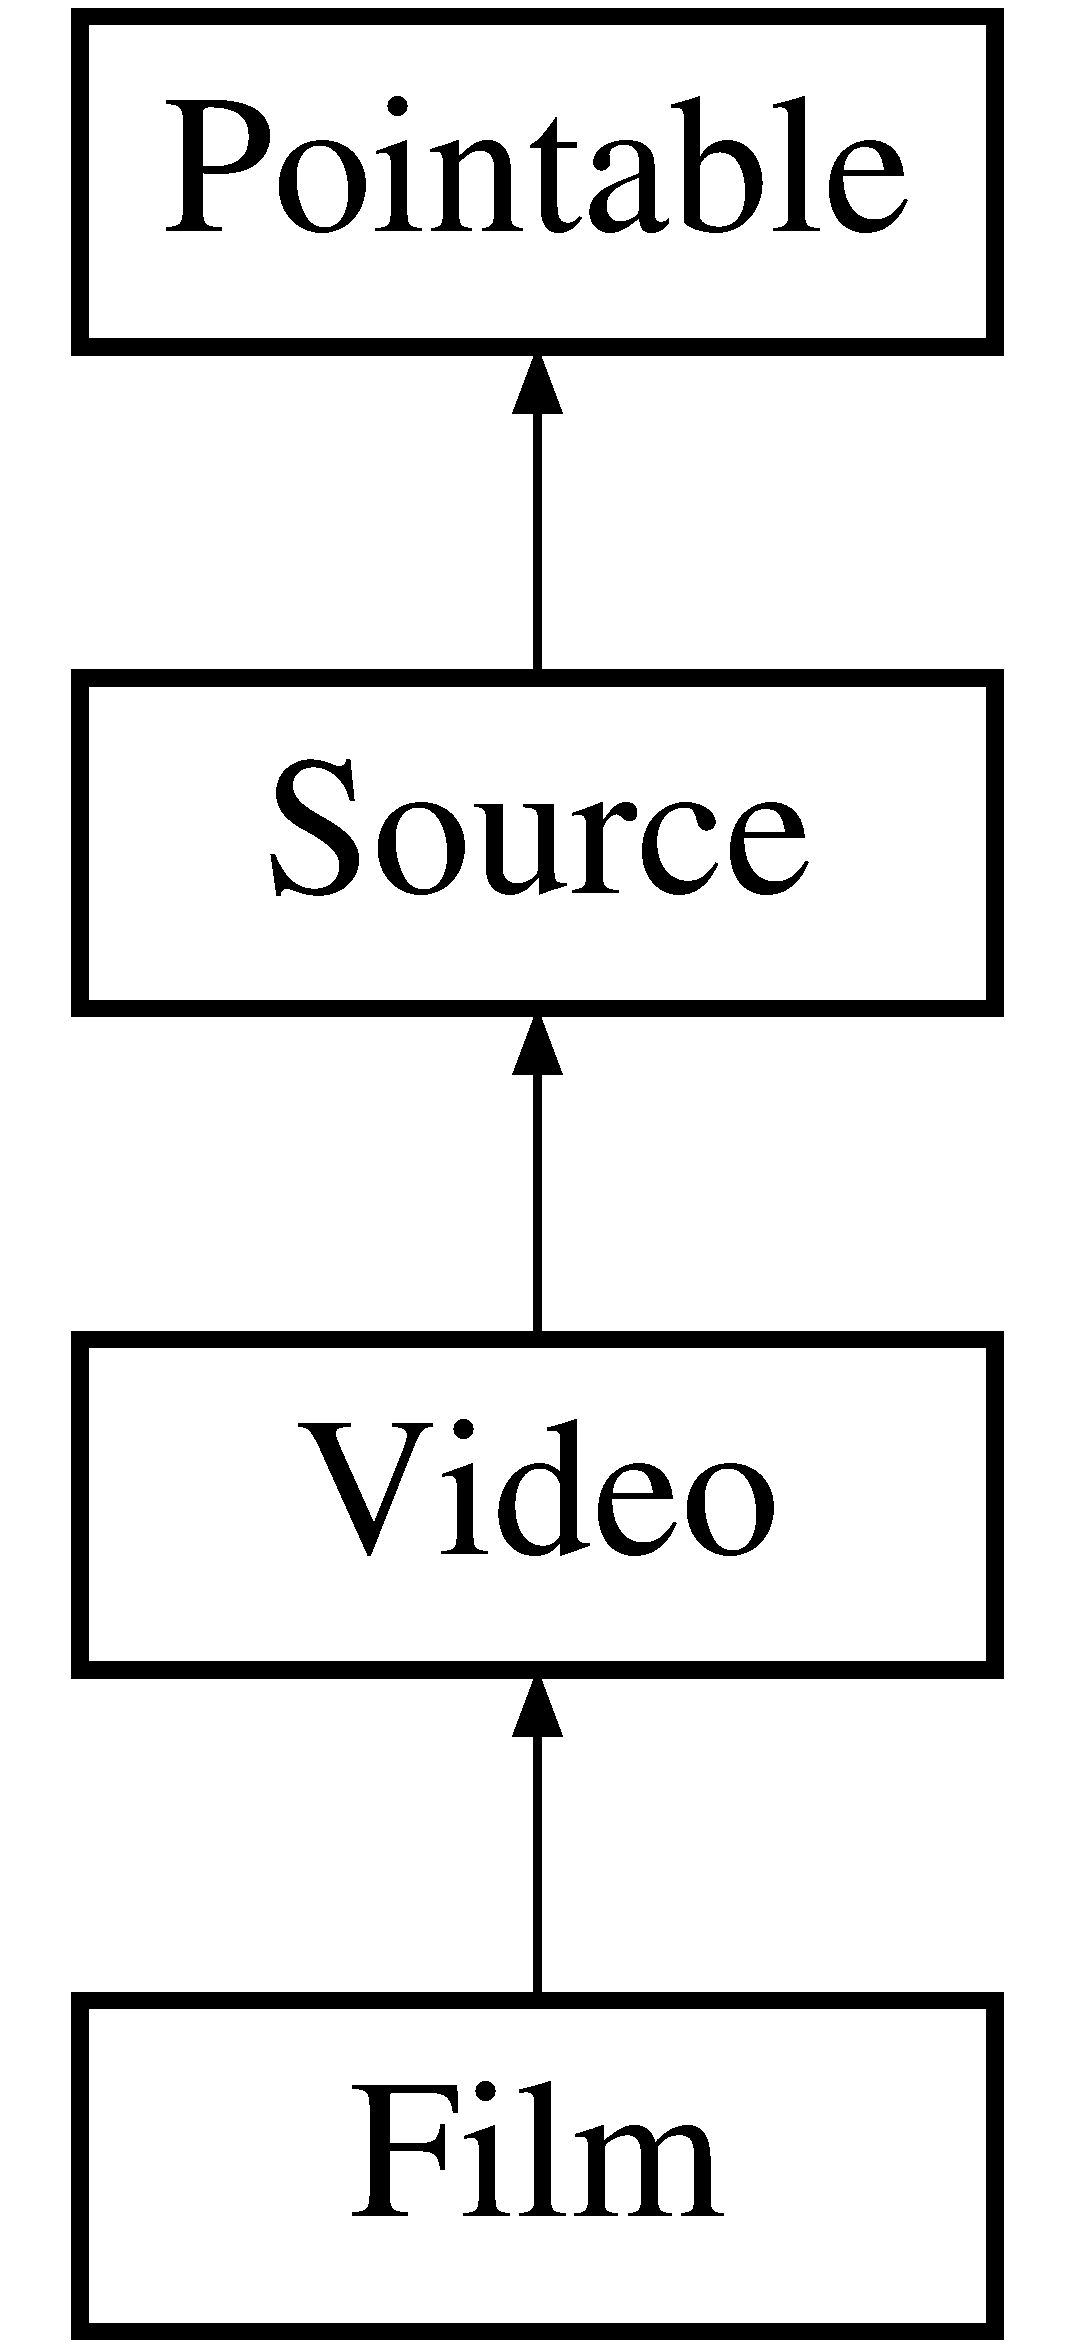
\includegraphics[height=4.000000cm]{classFilm}
\end{center}
\end{figure}
\subsection*{Public Member Functions}
\begin{DoxyCompactItemize}
\item 
\hypertarget{classFilm_af2835db2b0ef3a87aaa3222f4d9d1ae3}{\hyperlink{classFilm_af2835db2b0ef3a87aaa3222f4d9d1ae3}{Film} ()}\label{classFilm_af2835db2b0ef3a87aaa3222f4d9d1ae3}

\begin{DoxyCompactList}\small\item\em constructeur \end{DoxyCompactList}\item 
\hypertarget{classFilm_aa96dec38ef2e8db7fb03a68fc3d26da1}{{\bfseries Film} (string \-\_\-obj\-Name)}\label{classFilm_aa96dec38ef2e8db7fb03a68fc3d26da1}

\item 
\hypertarget{classFilm_a80fb97da0e99dffe97ea2eccc29c866f}{{\bfseries Film} (string \-\_\-obj\-Name, string path\-Prefix)}\label{classFilm_a80fb97da0e99dffe97ea2eccc29c866f}

\item 
\hypertarget{classFilm_a38f7d6e8e299bce1604f8300f60052f7}{{\bfseries Film} (string \-\_\-obj\-Name, string path\-Prefix, int \-\_\-dur)}\label{classFilm_a38f7d6e8e299bce1604f8300f60052f7}

\item 
\hypertarget{classFilm_a34c9de2efb9554ce1192e4110d98806b}{\hyperlink{classFilm_a34c9de2efb9554ce1192e4110d98806b}{Film} (const \hyperlink{classFilm}{Film} \&)}\label{classFilm_a34c9de2efb9554ce1192e4110d98806b}

\begin{DoxyCompactList}\small\item\em constructeur a partir d'une autre instance \end{DoxyCompactList}\item 
\hyperlink{classFilm}{Film} \& \hyperlink{classFilm_a2691ad8cf20210033cc35a6aa28e8553}{operator=} (const \hyperlink{classFilm}{Film} \&)
\begin{DoxyCompactList}\small\item\em redefinition de l'operateur = \end{DoxyCompactList}\item 
\hypertarget{classFilm_a8dab653f8a6c0635ca5ddbe0bbdd9a25}{virtual \hyperlink{classFilm_a8dab653f8a6c0635ca5ddbe0bbdd9a25}{$\sim$\-Film} ()}\label{classFilm_a8dab653f8a6c0635ca5ddbe0bbdd9a25}

\begin{DoxyCompactList}\small\item\em destructeur \end{DoxyCompactList}\item 
virtual void \hyperlink{classFilm_a27097a4f146d22c069f4ac429d40372d}{set\-Tab\-Dur} (const int $\ast$\-\_\-tab\-Dur, int size)
\begin{DoxyCompactList}\small\item\em setter \end{DoxyCompactList}\item 
virtual const int $\ast$ \hyperlink{classFilm_a3ac1dee35b575835c68e92bf64826618}{get\-Tab\-Dur} () const 
\begin{DoxyCompactList}\small\item\em getter du tableau de durees \end{DoxyCompactList}\item 
virtual int \hyperlink{classFilm_a0dfdcf162d9a84e965c22435ca146310}{get\-Nb\-Chap} () const 
\begin{DoxyCompactList}\small\item\em getter du nombre de chapitres \end{DoxyCompactList}\item 
\hypertarget{classFilm_a2dfafda0577fa5292674cb937eb7c6aa}{virtual void \hyperlink{classFilm_a2dfafda0577fa5292674cb937eb7c6aa}{print} () const }\label{classFilm_a2dfafda0577fa5292674cb937eb7c6aa}

\begin{DoxyCompactList}\small\item\em affichage \end{DoxyCompactList}\item 
\hypertarget{classFilm_a0fb4461cad5926a69443041887b21dbc}{virtual std\-::stringstream \& \hyperlink{classFilm_a0fb4461cad5926a69443041887b21dbc}{print\-To\-Stream} (stringstream \&stream) const }\label{classFilm_a0fb4461cad5926a69443041887b21dbc}

\begin{DoxyCompactList}\small\item\em ecrire la descriptio dans un stringstream \end{DoxyCompactList}\item 
\hypertarget{classFilm_a2da141229a61f420e3fc099124434700}{virtual void \hyperlink{classFilm_a2da141229a61f420e3fc099124434700}{play} () const }\label{classFilm_a2da141229a61f420e3fc099124434700}

\begin{DoxyCompactList}\small\item\em play \end{DoxyCompactList}\end{DoxyCompactItemize}
\subsection*{Additional Inherited Members}


\subsection{Detailed Description}
The \hyperlink{classFilm}{Film} class heritee de la classe \hyperlink{classVideo}{Video}. 

\subsection{Member Function Documentation}
\hypertarget{classFilm_a0dfdcf162d9a84e965c22435ca146310}{\index{Film@{Film}!get\-Nb\-Chap@{get\-Nb\-Chap}}
\index{get\-Nb\-Chap@{get\-Nb\-Chap}!Film@{Film}}
\subsubsection[{get\-Nb\-Chap}]{\setlength{\rightskip}{0pt plus 5cm}int Film\-::get\-Nb\-Chap (
\begin{DoxyParamCaption}
{}
\end{DoxyParamCaption}
) const\hspace{0.3cm}{\ttfamily [virtual]}}}\label{classFilm_a0dfdcf162d9a84e965c22435ca146310}


getter du nombre de chapitres 

get nombre de chapitres \hypertarget{classFilm_a3ac1dee35b575835c68e92bf64826618}{\index{Film@{Film}!get\-Tab\-Dur@{get\-Tab\-Dur}}
\index{get\-Tab\-Dur@{get\-Tab\-Dur}!Film@{Film}}
\subsubsection[{get\-Tab\-Dur}]{\setlength{\rightskip}{0pt plus 5cm}const int $\ast$ Film\-::get\-Tab\-Dur (
\begin{DoxyParamCaption}
{}
\end{DoxyParamCaption}
) const\hspace{0.3cm}{\ttfamily [virtual]}}}\label{classFilm_a3ac1dee35b575835c68e92bf64826618}


getter du tableau de durees 

getter \hypertarget{classFilm_a2691ad8cf20210033cc35a6aa28e8553}{\index{Film@{Film}!operator=@{operator=}}
\index{operator=@{operator=}!Film@{Film}}
\subsubsection[{operator=}]{\setlength{\rightskip}{0pt plus 5cm}{\bf Film} \& Film\-::operator= (
\begin{DoxyParamCaption}
\item[{const {\bf Film} \&}]{from}
\end{DoxyParamCaption}
)}}\label{classFilm_a2691ad8cf20210033cc35a6aa28e8553}


redefinition de l'operateur = 

redefinition de l'operateur =, copie profonde \hypertarget{classFilm_a27097a4f146d22c069f4ac429d40372d}{\index{Film@{Film}!set\-Tab\-Dur@{set\-Tab\-Dur}}
\index{set\-Tab\-Dur@{set\-Tab\-Dur}!Film@{Film}}
\subsubsection[{set\-Tab\-Dur}]{\setlength{\rightskip}{0pt plus 5cm}void Film\-::set\-Tab\-Dur (
\begin{DoxyParamCaption}
\item[{const int $\ast$}]{\-\_\-tab\-Dur, }
\item[{int}]{size}
\end{DoxyParamCaption}
)\hspace{0.3cm}{\ttfamily [virtual]}}}\label{classFilm_a27097a4f146d22c069f4ac429d40372d}


setter 

setter, copie d'un tableau de duree 

The documentation for this class was generated from the following files\-:\begin{DoxyCompactItemize}
\item 
film.\-h\item 
film.\-cpp\end{DoxyCompactItemize}

\hypertarget{classGroupe}{\section{Groupe Class Reference}
\label{classGroupe}\index{Groupe@{Groupe}}
}


The \hyperlink{classGroupe}{Groupe} class class heritee de std\-::list.  




{\ttfamily \#include $<$groupe.\-h$>$}

Inheritance diagram for Groupe\-:\begin{figure}[H]
\begin{center}
\leavevmode
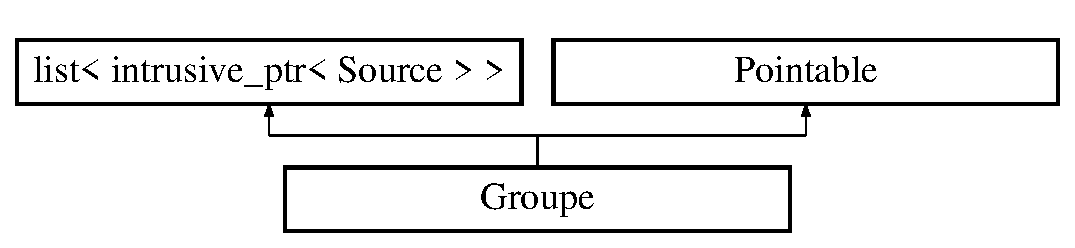
\includegraphics[height=2.000000cm]{classGroupe}
\end{center}
\end{figure}
\subsection*{Public Member Functions}
\begin{DoxyCompactItemize}
\item 
\hypertarget{classGroupe_ad4cd49f43b43c2a0abfc7b283f37e9bc}{\hyperlink{classGroupe_ad4cd49f43b43c2a0abfc7b283f37e9bc}{Groupe} (string \-\_\-name)}\label{classGroupe_ad4cd49f43b43c2a0abfc7b283f37e9bc}

\begin{DoxyCompactList}\small\item\em constructeur, donner le nom du groupe \end{DoxyCompactList}\item 
\hypertarget{classGroupe_a99dd414922635dcc0585aabb2a330f63}{virtual \hyperlink{classGroupe_a99dd414922635dcc0585aabb2a330f63}{$\sim$\-Groupe} ()}\label{classGroupe_a99dd414922635dcc0585aabb2a330f63}

\begin{DoxyCompactList}\small\item\em destructeur \end{DoxyCompactList}\item 
\hypertarget{classGroupe_a37f0f8e74f1826265933503de8a45583}{virtual string \hyperlink{classGroupe_a37f0f8e74f1826265933503de8a45583}{get\-Group\-Name} () const }\label{classGroupe_a37f0f8e74f1826265933503de8a45583}

\begin{DoxyCompactList}\small\item\em getter du nom du groupe \end{DoxyCompactList}\item 
\hypertarget{classGroupe_aaf187c7b1df6740b05cae4e504a83874}{virtual void \hyperlink{classGroupe_aaf187c7b1df6740b05cae4e504a83874}{print} () const }\label{classGroupe_aaf187c7b1df6740b05cae4e504a83874}

\begin{DoxyCompactList}\small\item\em affichage des elements dans le groupe \end{DoxyCompactList}\end{DoxyCompactItemize}


\subsection{Detailed Description}
The \hyperlink{classGroupe}{Groupe} class class heritee de std\-::list. 

The documentation for this class was generated from the following files\-:\begin{DoxyCompactItemize}
\item 
groupe.\-h\item 
groupe.\-cpp\end{DoxyCompactItemize}

\hypertarget{structTCPServer_1_1Hook}{\section{T\-C\-P\-Server\-:\-:Hook Struct Reference}
\label{structTCPServer_1_1Hook}\index{T\-C\-P\-Server\-::\-Hook@{T\-C\-P\-Server\-::\-Hook}}
}
\subsection*{Public Member Functions}
\begin{DoxyCompactItemize}
\item 
\hypertarget{structTCPServer_1_1Hook_ab7d1f34003d7e1351802b78d70513b69}{{\bfseries Hook} (\hyperlink{classTCPServer}{T\-C\-P\-Server} $\ast$\-\_\-server, \hyperlink{classSocket}{Socket} $\ast$\-\_\-sock)}\label{structTCPServer_1_1Hook_ab7d1f34003d7e1351802b78d70513b69}

\end{DoxyCompactItemize}
\subsection*{Public Attributes}
\begin{DoxyCompactItemize}
\item 
\hypertarget{structTCPServer_1_1Hook_a05a2a91ba8cd71e45a702160842f9025}{\hyperlink{classTCPServer}{T\-C\-P\-Server} $\ast$ {\bfseries server}}\label{structTCPServer_1_1Hook_a05a2a91ba8cd71e45a702160842f9025}

\item 
\hypertarget{structTCPServer_1_1Hook_a511a47e58128074e7aa9992371fbdd1e}{\hyperlink{classSocket}{Socket} $\ast$ {\bfseries sock}}\label{structTCPServer_1_1Hook_a511a47e58128074e7aa9992371fbdd1e}

\end{DoxyCompactItemize}


The documentation for this struct was generated from the following file\-:\begin{DoxyCompactItemize}
\item 
T\-C\-P\-Server.\-h\end{DoxyCompactItemize}

\hypertarget{classintrusive__ptr}{\section{intrusive\-\_\-ptr$<$ T $>$ Class Template Reference}
\label{classintrusive__ptr}\index{intrusive\-\_\-ptr$<$ T $>$@{intrusive\-\_\-ptr$<$ T $>$}}
}


{\ttfamily \#include $<$intrusive\-\_\-ptr.\-h$>$}

\subsection*{Public Types}
\begin{DoxyCompactItemize}
\item 
\hypertarget{classintrusive__ptr_ae15c9aa35038587012d1b08729cc19c9}{typedef T {\bfseries element\-\_\-type}}\label{classintrusive__ptr_ae15c9aa35038587012d1b08729cc19c9}

\end{DoxyCompactItemize}
\subsection*{Public Member Functions}
\begin{DoxyCompactItemize}
\item 
\hypertarget{classintrusive__ptr_a1a462a7c6f3247828d8360ca04511237}{{\bfseries intrusive\-\_\-ptr} (T $\ast$p, bool add\-\_\-ref=true)}\label{classintrusive__ptr_a1a462a7c6f3247828d8360ca04511237}

\item 
\hypertarget{classintrusive__ptr_a60d33e3607b90c2d7f315d2d0be19735}{{\footnotesize template$<$class U $>$ }\\{\bfseries intrusive\-\_\-ptr} (\hyperlink{classintrusive__ptr}{intrusive\-\_\-ptr}$<$ U $>$ const \&rhs)}\label{classintrusive__ptr_a60d33e3607b90c2d7f315d2d0be19735}

\item 
\hypertarget{classintrusive__ptr_a1a05008b03d6cfb92dfa60515cd848d8}{{\bfseries intrusive\-\_\-ptr} (\hyperlink{classintrusive__ptr}{intrusive\-\_\-ptr} const \&rhs)}\label{classintrusive__ptr_a1a05008b03d6cfb92dfa60515cd848d8}

\item 
\hypertarget{classintrusive__ptr_a3f784a56085dd6e9f711e57a803dd1dc}{{\footnotesize template$<$class U $>$ }\\\hyperlink{classintrusive__ptr}{intrusive\-\_\-ptr} \& {\bfseries operator=} (\hyperlink{classintrusive__ptr}{intrusive\-\_\-ptr}$<$ U $>$ const \&rhs)}\label{classintrusive__ptr_a3f784a56085dd6e9f711e57a803dd1dc}

\item 
\hypertarget{classintrusive__ptr_ae1f058e2b20ea4ef7c3c4c30c8c37694}{\hyperlink{classintrusive__ptr}{intrusive\-\_\-ptr} \& {\bfseries operator=} (\hyperlink{classintrusive__ptr}{intrusive\-\_\-ptr} const \&rhs)}\label{classintrusive__ptr_ae1f058e2b20ea4ef7c3c4c30c8c37694}

\item 
\hypertarget{classintrusive__ptr_acbf9dbecf8e789db853832d84e2c7e19}{\hyperlink{classintrusive__ptr}{intrusive\-\_\-ptr} \& {\bfseries operator=} (T $\ast$rhs)}\label{classintrusive__ptr_acbf9dbecf8e789db853832d84e2c7e19}

\item 
\hypertarget{classintrusive__ptr_ae360b0fffd335b683b350c154922c6db}{void {\bfseries reset} ()}\label{classintrusive__ptr_ae360b0fffd335b683b350c154922c6db}

\item 
\hypertarget{classintrusive__ptr_a81e2fb688afba02de9ecf2006caeb62e}{void {\bfseries reset} (T $\ast$rhs)}\label{classintrusive__ptr_a81e2fb688afba02de9ecf2006caeb62e}

\item 
\hypertarget{classintrusive__ptr_a70192c07e3ff5035942095a5d2d97c34}{T $\ast$ {\bfseries get} () const }\label{classintrusive__ptr_a70192c07e3ff5035942095a5d2d97c34}

\item 
\hypertarget{classintrusive__ptr_a63f7f0b02c547127f9f68ecdb01f7aa6}{T \& {\bfseries operator$\ast$} () const }\label{classintrusive__ptr_a63f7f0b02c547127f9f68ecdb01f7aa6}

\item 
\hypertarget{classintrusive__ptr_a4756c9e89a1a057e2c911d8224197d31}{T $\ast$ {\bfseries operator-\/$>$} () const }\label{classintrusive__ptr_a4756c9e89a1a057e2c911d8224197d31}

\item 
\hypertarget{classintrusive__ptr_a1a71711829594617e226fada9b7ef351}{{\bfseries operator unspecified\-\_\-bool\-\_\-type} () const }\label{classintrusive__ptr_a1a71711829594617e226fada9b7ef351}

\item 
\hypertarget{classintrusive__ptr_aee167762c6829dac96f664b4ab505e39}{bool {\bfseries operator!} () const }\label{classintrusive__ptr_aee167762c6829dac96f664b4ab505e39}

\item 
\hypertarget{classintrusive__ptr_a95826a79f706bc5c6b9fd28ae334e974}{void {\bfseries swap} (\hyperlink{classintrusive__ptr}{intrusive\-\_\-ptr} \&rhs)}\label{classintrusive__ptr_a95826a79f706bc5c6b9fd28ae334e974}

\end{DoxyCompactItemize}


\subsection{Detailed Description}
\subsubsection*{template$<$class T$>$class intrusive\-\_\-ptr$<$ T $>$}

\hyperlink{classintrusive__ptr}{intrusive\-\_\-ptr}\-: a smart pointer that uses intrusive reference counting. Relies on unqualified calls to 
\begin{DoxyPre}
     void intrusive\_ptr\_add\_ref(T * p);
     void intrusive\_ptr\_release(T * p);
\end{DoxyPre}
 (p != 0)

The object is responsible for destroying itself. 

The documentation for this class was generated from the following file\-:\begin{DoxyCompactItemize}
\item 
intrusive\-\_\-ptr.\-h\end{DoxyCompactItemize}

\hypertarget{classPhoto}{\section{Photo Class Reference}
\label{classPhoto}\index{Photo@{Photo}}
}


The \hyperlink{classPhoto}{Photo} class heritee de la classe \hyperlink{classSource}{Source}.  




{\ttfamily \#include $<$photo.\-h$>$}

Inheritance diagram for Photo\-:\begin{figure}[H]
\begin{center}
\leavevmode
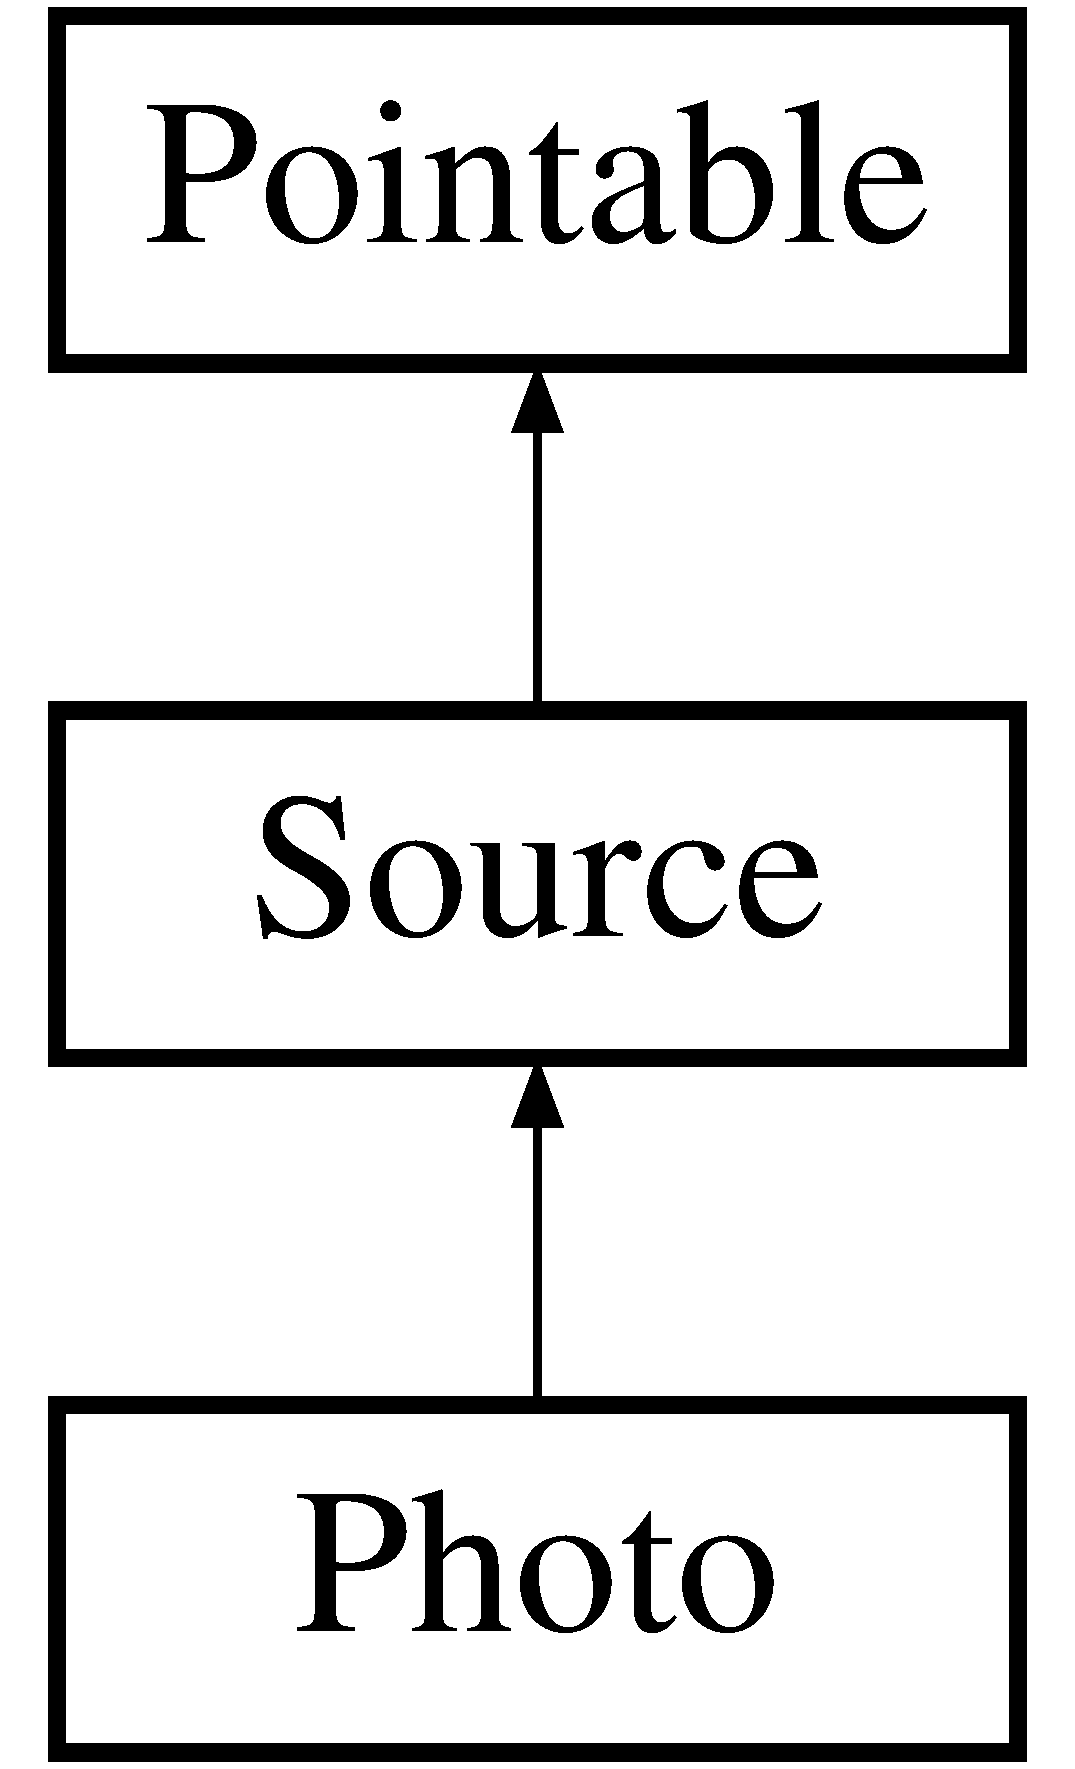
\includegraphics[height=3.000000cm]{classPhoto}
\end{center}
\end{figure}
\subsection*{Public Member Functions}
\begin{DoxyCompactItemize}
\item 
\hypertarget{classPhoto_a10ef03ede9235052eb9f7d5e950f85d3}{\hyperlink{classPhoto_a10ef03ede9235052eb9f7d5e950f85d3}{Photo} ()}\label{classPhoto_a10ef03ede9235052eb9f7d5e950f85d3}

\begin{DoxyCompactList}\small\item\em constructeur \end{DoxyCompactList}\item 
\hypertarget{classPhoto_aa8b1ff45e4ce396b16feed0359fee5d1}{{\bfseries Photo} (string \-\_\-obj\-Name)}\label{classPhoto_aa8b1ff45e4ce396b16feed0359fee5d1}

\item 
\hypertarget{classPhoto_a34c737e6e1f77dc9d3ba7e03bfad11bb}{{\bfseries Photo} (string \-\_\-obj\-Name, string path\-Prefix)}\label{classPhoto_a34c737e6e1f77dc9d3ba7e03bfad11bb}

\item 
\hypertarget{classPhoto_adc366234be6226600360c7cbba8e7fcf}{virtual \hyperlink{classPhoto_adc366234be6226600360c7cbba8e7fcf}{$\sim$\-Photo} ()}\label{classPhoto_adc366234be6226600360c7cbba8e7fcf}

\begin{DoxyCompactList}\small\item\em destructeur \end{DoxyCompactList}\item 
\hypertarget{classPhoto_a412f7dfbfe6c1bb6ef19d3d0067322d5}{virtual string \hyperlink{classPhoto_a412f7dfbfe6c1bb6ef19d3d0067322d5}{get\-Place} () const }\label{classPhoto_a412f7dfbfe6c1bb6ef19d3d0067322d5}

\begin{DoxyCompactList}\small\item\em getter \end{DoxyCompactList}\item 
\hypertarget{classPhoto_ab01ceff1921d80a260659f775b7d68e9}{virtual void \hyperlink{classPhoto_ab01ceff1921d80a260659f775b7d68e9}{set\-Place} (string \-\_\-place)}\label{classPhoto_ab01ceff1921d80a260659f775b7d68e9}

\begin{DoxyCompactList}\small\item\em setter \end{DoxyCompactList}\item 
\hypertarget{classPhoto_a172eee7d20b6852a4bc2c4ec5494610f}{virtual void \hyperlink{classPhoto_a172eee7d20b6852a4bc2c4ec5494610f}{print} () const }\label{classPhoto_a172eee7d20b6852a4bc2c4ec5494610f}

\begin{DoxyCompactList}\small\item\em affichage \end{DoxyCompactList}\item 
\hypertarget{classPhoto_aea46b6547f584c315a5150637ebf5c36}{virtual std\-::stringstream \& \hyperlink{classPhoto_aea46b6547f584c315a5150637ebf5c36}{print\-To\-Stream} (stringstream \&stream) const }\label{classPhoto_aea46b6547f584c315a5150637ebf5c36}

\begin{DoxyCompactList}\small\item\em ecrire dans un stringstream \end{DoxyCompactList}\item 
\hypertarget{classPhoto_a34ef1c73e123d2951e8a08b3b1697c05}{virtual void \hyperlink{classPhoto_a34ef1c73e123d2951e8a08b3b1697c05}{play} () const }\label{classPhoto_a34ef1c73e123d2951e8a08b3b1697c05}

\begin{DoxyCompactList}\small\item\em play \end{DoxyCompactList}\end{DoxyCompactItemize}
\subsection*{Protected Attributes}
\begin{DoxyCompactItemize}
\item 
\hypertarget{classPhoto_aa5eebcbcc98061b25d054417e120c411}{string {\bfseries place}}\label{classPhoto_aa5eebcbcc98061b25d054417e120c411}

\end{DoxyCompactItemize}


\subsection{Detailed Description}
The \hyperlink{classPhoto}{Photo} class heritee de la classe \hyperlink{classSource}{Source}. 

The documentation for this class was generated from the following files\-:\begin{DoxyCompactItemize}
\item 
photo.\-h\item 
photo.\-cpp\end{DoxyCompactItemize}

\hypertarget{classPointable}{\section{Pointable Class Reference}
\label{classPointable}\index{Pointable@{Pointable}}
}


{\ttfamily \#include $<$intrusive\-\_\-ptr.\-h$>$}

Inheritance diagram for Pointable\-:\begin{figure}[H]
\begin{center}
\leavevmode
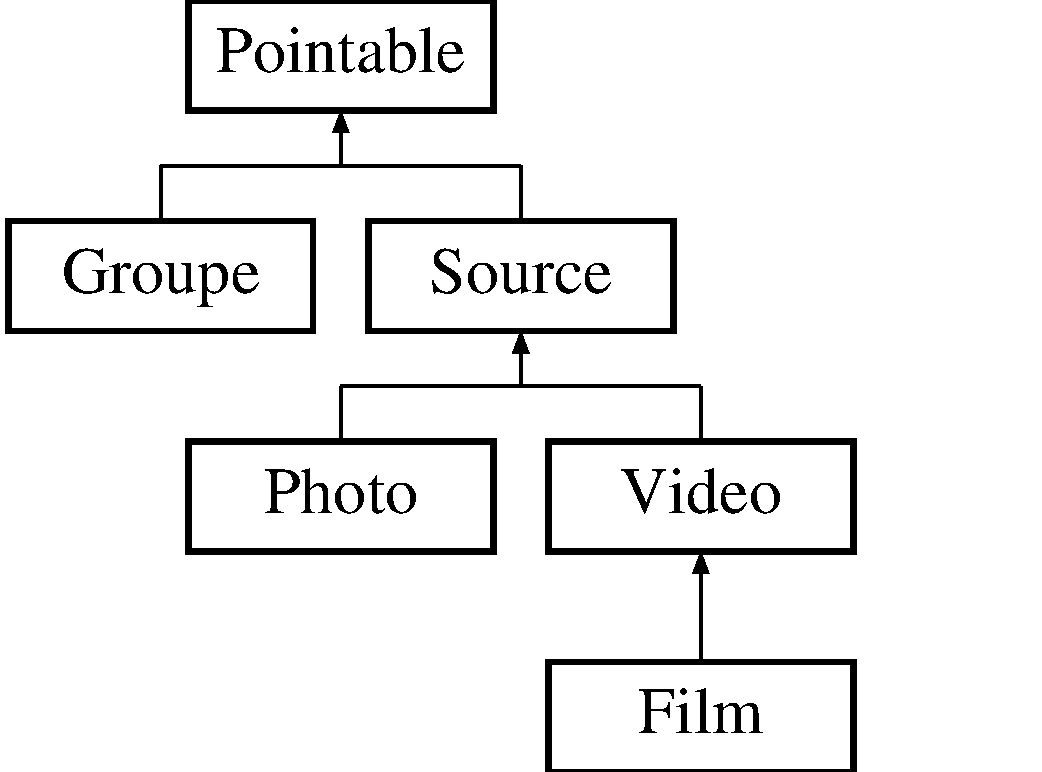
\includegraphics[height=4.000000cm]{classPointable}
\end{center}
\end{figure}
\subsection*{Public Member Functions}
\begin{DoxyCompactItemize}
\item 
\hypertarget{classPointable_adc4da364054bdd4c4a9624f5dc190c8a}{{\bfseries Pointable} (const \hyperlink{classPointable}{Pointable} \&)}\label{classPointable_adc4da364054bdd4c4a9624f5dc190c8a}

\item 
\hypertarget{classPointable_a8a7eb6956905e6e320ce97fa24f03b59}{\hyperlink{classPointable}{Pointable} \& {\bfseries operator=} (const \hyperlink{classPointable}{Pointable} \&)}\label{classPointable_a8a7eb6956905e6e320ce97fa24f03b59}

\item 
\hypertarget{classPointable_a48c9c705dd509cdafc2663b092865120}{long {\bfseries get\-Count} ()}\label{classPointable_a48c9c705dd509cdafc2663b092865120}

\end{DoxyCompactItemize}
\subsection*{Friends}
\begin{DoxyCompactItemize}
\item 
\hypertarget{classPointable_a9c08ce04af1d8cd2697b64990c51a5f4}{long {\bfseries intrusive\-\_\-ptr\-\_\-get\-\_\-count} (\hyperlink{classPointable}{Pointable} $\ast$p)}\label{classPointable_a9c08ce04af1d8cd2697b64990c51a5f4}

\item 
\hypertarget{classPointable_a16ec5f964af06a93d6c7cfe0979ff672}{void {\bfseries intrusive\-\_\-ptr\-\_\-add\-\_\-ref} (\hyperlink{classPointable}{Pointable} $\ast$p)}\label{classPointable_a16ec5f964af06a93d6c7cfe0979ff672}

\item 
\hypertarget{classPointable_aee25e5a73726af47eb078e2087eaee57}{void {\bfseries intrusive\-\_\-ptr\-\_\-release} (\hyperlink{classPointable}{Pointable} $\ast$p)}\label{classPointable_aee25e5a73726af47eb078e2087eaee57}

\end{DoxyCompactItemize}


\subsection{Detailed Description}
Generic base class for objects that can be pointed by an \hyperlink{classintrusive__ptr}{intrusive\-\_\-ptr}.
\begin{DoxyItemize}
\item \begin{DoxySeeAlso}{See Also}
\hyperlink{classintrusive__ptr}{intrusive\-\_\-ptr} for details
\end{DoxySeeAlso}

\item misc. checkings are performed if macro S\-M\-A\-R\-T\-\_\-\-P\-T\-R\-\_\-\-D\-E\-B\-U\-G is defined before including \hyperlink{intrusive__ptr_8h_source}{intrusive\-\_\-ptr.\-h}
\item debug messages are displayed on stderr if macros S\-M\-A\-R\-T\-\_\-\-P\-T\-R\-\_\-\-D\-E\-B\-U\-G and if S\-M\-A\-R\-T\-\_\-\-P\-T\-R\-\_\-\-D\-E\-B\-U\-G\-\_\-\-M\-E\-S\-S\-A\-G\-E\-S are both defined. 
\end{DoxyItemize}

The documentation for this class was generated from the following file\-:\begin{DoxyCompactItemize}
\item 
intrusive\-\_\-ptr.\-h\end{DoxyCompactItemize}

\hypertarget{classServerSocket}{\section{Server\-Socket Class Reference}
\label{classServerSocket}\index{Server\-Socket@{Server\-Socket}}
}


{\ttfamily \#include $<$Socket.\-h$>$}

\subsection*{Public Member Functions}
\begin{DoxyCompactItemize}
\item 
\hyperlink{classServerSocket_a668d35aeea12aafa0025ecbc6313113f}{Server\-Socket} (int type=S\-O\-C\-K\-\_\-\-S\-T\-R\-E\-A\-M)
\item 
virtual \hyperlink{classSocket}{Socket} $\ast$ \hyperlink{classServerSocket_accc3d56d42aa50a5f3c920cf0b26959b}{accept} ()
\item 
virtual int \hyperlink{classServerSocket_ad5281fe6c005bca007a9a758bd612481}{bind} (int port, int backlog=50)
\item 
\hypertarget{classServerSocket_a3eac6d5571bb092622d328dbda2de2cf}{virtual int \hyperlink{classServerSocket_a3eac6d5571bb092622d328dbda2de2cf}{close} ()}\label{classServerSocket_a3eac6d5571bb092622d328dbda2de2cf}

\begin{DoxyCompactList}\small\item\em closes the socket. \end{DoxyCompactList}\item 
\hypertarget{classServerSocket_a73a32b4697d3ff2bc9a68700f06e4dfb}{int \hyperlink{classServerSocket_a73a32b4697d3ff2bc9a68700f06e4dfb}{get\-File\-Descriptor} () const }\label{classServerSocket_a73a32b4697d3ff2bc9a68700f06e4dfb}

\begin{DoxyCompactList}\small\item\em returns the file descriptor of the socket. \end{DoxyCompactList}\item 
void \hyperlink{classServerSocket_afe81d7c30d1e963e6a043b868560dbbd}{handle\-Sig\-Pipe} (void($\ast$function)(int signal))
\item 
void \hyperlink{classServerSocket_ac159a12414df54dfef149a8de6aacb20}{ignore\-Sig\-Pipe} ()
\begin{DoxyCompactList}\small\item\em ignore S\-I\-G\-P\-I\-P\-E signals ( \end{DoxyCompactList}\item 
int \hyperlink{classServerSocket_a7ad8a5581c52046e641b32d96eb23406}{get\-Option} (int level, int optname, void $\ast$optval, socklen\-\_\-t $\ast$optlen)
\item 
int \hyperlink{classServerSocket_ad69fa5c5891f028192a291044b9191e2}{set\-Option} (int level, int optname, const void $\ast$optval, socklen\-\_\-t optlen)
\item 
\hypertarget{classServerSocket_ab34154bc6114c638ae02f5e018121099}{int \hyperlink{classServerSocket_ab34154bc6114c638ae02f5e018121099}{set\-Receive\-Buffer\-Size} (int size)}\label{classServerSocket_ab34154bc6114c638ae02f5e018121099}

\begin{DoxyCompactList}\small\item\em sets the S\-O\-\_\-\-R\-C\-V\-B\-U\-F option to the specified value. \end{DoxyCompactList}\item 
\hypertarget{classServerSocket_ae60d7cc31ad535e5d3cac42e38b8ec98}{int \hyperlink{classServerSocket_ae60d7cc31ad535e5d3cac42e38b8ec98}{set\-Reuse\-Address} (bool)}\label{classServerSocket_ae60d7cc31ad535e5d3cac42e38b8ec98}

\begin{DoxyCompactList}\small\item\em enables/disables the S\-O\-\_\-\-R\-E\-U\-S\-E\-A\-D\-D\-R socket option. \end{DoxyCompactList}\item 
\hypertarget{classServerSocket_aedb9144c9c375fcb14ac47bcb9d2eb17}{int \hyperlink{classServerSocket_aedb9144c9c375fcb14ac47bcb9d2eb17}{set\-So\-Timeout} (int timeout)}\label{classServerSocket_aedb9144c9c375fcb14ac47bcb9d2eb17}

\begin{DoxyCompactList}\small\item\em enables/disables S\-O\-\_\-\-T\-I\-M\-E\-O\-U\-T with the specified timeout (in milliseconds). \end{DoxyCompactList}\item 
\hypertarget{classServerSocket_a9e5e1ee852ba26156c757a0086b780fe}{int \hyperlink{classServerSocket_a9e5e1ee852ba26156c757a0086b780fe}{set\-Tcp\-No\-Delay} (bool)}\label{classServerSocket_a9e5e1ee852ba26156c757a0086b780fe}

\begin{DoxyCompactList}\small\item\em turns on/off T\-C\-P coalescence (useful in some cases to avoid delays). \end{DoxyCompactList}\end{DoxyCompactItemize}


\subsection{Detailed Description}
T\-C\-P/\-I\-P or Datagram I\-N\-E\-T socket server. 

\subsection{Constructor \& Destructor Documentation}
\hypertarget{classServerSocket_a668d35aeea12aafa0025ecbc6313113f}{\index{Server\-Socket@{Server\-Socket}!Server\-Socket@{Server\-Socket}}
\index{Server\-Socket@{Server\-Socket}!ServerSocket@{Server\-Socket}}
\subsubsection[{Server\-Socket}]{\setlength{\rightskip}{0pt plus 5cm}Server\-Socket\-::\-Server\-Socket (
\begin{DoxyParamCaption}
\item[{int}]{type = {\ttfamily SOCK\-\_\-STREAM}}
\end{DoxyParamCaption}
)}}\label{classServerSocket_a668d35aeea12aafa0025ecbc6313113f}
creates a new \hyperlink{classServerSocket}{Server\-Socket}. Creates a listening A\-F\-\_\-\-I\-N\-E\-T socket (using the I\-Pv4 Internet protocol) that waits for connection requests by client sockets. 'type' can be\-:
\begin{DoxyItemize}
\item S\-O\-C\-K\-\_\-\-S\-T\-R\-E\-A\-M (the default) for T\-C\-P/\-I\-P connected sockets
\item S\-O\-C\-K\-\_\-\-D\-G\-R\-A\-M for U\-D\-P datagram sockets 
\end{DoxyItemize}

\subsection{Member Function Documentation}
\hypertarget{classServerSocket_accc3d56d42aa50a5f3c920cf0b26959b}{\index{Server\-Socket@{Server\-Socket}!accept@{accept}}
\index{accept@{accept}!ServerSocket@{Server\-Socket}}
\subsubsection[{accept}]{\setlength{\rightskip}{0pt plus 5cm}{\bf Socket} $\ast$ Server\-Socket\-::accept (
\begin{DoxyParamCaption}
{}
\end{DoxyParamCaption}
)\hspace{0.3cm}{\ttfamily [virtual]}}}\label{classServerSocket_accc3d56d42aa50a5f3c920cf0b26959b}
accepts a new connection request and returns the corresponding socket. By default, this function blocks the caller until a connection is present \begin{DoxyReturn}{Returns}
Returns the new \hyperlink{classSocket}{Socket} or N\-U\-L\-L on error 
\end{DoxyReturn}
\hypertarget{classServerSocket_ad5281fe6c005bca007a9a758bd612481}{\index{Server\-Socket@{Server\-Socket}!bind@{bind}}
\index{bind@{bind}!ServerSocket@{Server\-Socket}}
\subsubsection[{bind}]{\setlength{\rightskip}{0pt plus 5cm}int Server\-Socket\-::bind (
\begin{DoxyParamCaption}
\item[{int}]{port, }
\item[{int}]{backlog = {\ttfamily 50}}
\end{DoxyParamCaption}
)\hspace{0.3cm}{\ttfamily [virtual]}}}\label{classServerSocket_ad5281fe6c005bca007a9a758bd612481}
assigns this port to the socket on localhost. \begin{DoxyReturn}{Returns}
returns 0 on success or a negative value on error which is one of\-:
\begin{DoxyItemize}
\item Socket\-::\-F\-A\-I\-L\-E\-D (-\/1)\-: could not connect
\item Socket\-::\-I\-N\-V\-A\-L\-I\-D\-\_\-\-S\-O\-C\-K\-E\-T\-: wrong socket type. 
\end{DoxyItemize}
\end{DoxyReturn}
\hypertarget{classServerSocket_a7ad8a5581c52046e641b32d96eb23406}{\index{Server\-Socket@{Server\-Socket}!get\-Option@{get\-Option}}
\index{get\-Option@{get\-Option}!ServerSocket@{Server\-Socket}}
\subsubsection[{get\-Option}]{\setlength{\rightskip}{0pt plus 5cm}int Server\-Socket\-::get\-Option (
\begin{DoxyParamCaption}
\item[{int}]{level, }
\item[{int}]{optname, }
\item[{void $\ast$}]{optval, }
\item[{socklen\-\_\-t $\ast$}]{optlen}
\end{DoxyParamCaption}
)}}\label{classServerSocket_a7ad8a5581c52046e641b32d96eb23406}
gets socket options. Same arguments and effect as the getsockopt() system call. \begin{DoxyReturn}{Returns}
On success, zero is returned. On error, -\/1 is returned. 
\end{DoxyReturn}
\hypertarget{classServerSocket_afe81d7c30d1e963e6a043b868560dbbd}{\index{Server\-Socket@{Server\-Socket}!handle\-Sig\-Pipe@{handle\-Sig\-Pipe}}
\index{handle\-Sig\-Pipe@{handle\-Sig\-Pipe}!ServerSocket@{Server\-Socket}}
\subsubsection[{handle\-Sig\-Pipe}]{\setlength{\rightskip}{0pt plus 5cm}void Server\-Socket\-::handle\-Sig\-Pipe (
\begin{DoxyParamCaption}
\item[{void($\ast$)(int signal)}]{function}
\end{DoxyParamCaption}
)}}\label{classServerSocket_afe81d7c30d1e963e6a043b868560dbbd}
handle S\-I\-G\-P\-I\-P\-E signals. Sockets may abort programs by throwing a S\-I\-G\-P\-I\-P\-E signal. The function given as an argument will be called instead of aborting the program.  \hyperlink{classServerSocket_ac159a12414df54dfef149a8de6aacb20}{ignore\-Sig\-Pipe()} \hypertarget{classServerSocket_ac159a12414df54dfef149a8de6aacb20}{\index{Server\-Socket@{Server\-Socket}!ignore\-Sig\-Pipe@{ignore\-Sig\-Pipe}}
\index{ignore\-Sig\-Pipe@{ignore\-Sig\-Pipe}!ServerSocket@{Server\-Socket}}
\subsubsection[{ignore\-Sig\-Pipe}]{\setlength{\rightskip}{0pt plus 5cm}void Server\-Socket\-::ignore\-Sig\-Pipe (
\begin{DoxyParamCaption}
{}
\end{DoxyParamCaption}
)}}\label{classServerSocket_ac159a12414df54dfef149a8de6aacb20}


ignore S\-I\-G\-P\-I\-P\-E signals ( 

\begin{DoxySeeAlso}{See Also}
\hyperlink{classServerSocket_afe81d7c30d1e963e6a043b868560dbbd}{handle\-Sig\-Pipe()}). 
\end{DoxySeeAlso}
\hypertarget{classServerSocket_ad69fa5c5891f028192a291044b9191e2}{\index{Server\-Socket@{Server\-Socket}!set\-Option@{set\-Option}}
\index{set\-Option@{set\-Option}!ServerSocket@{Server\-Socket}}
\subsubsection[{set\-Option}]{\setlength{\rightskip}{0pt plus 5cm}int Server\-Socket\-::set\-Option (
\begin{DoxyParamCaption}
\item[{int}]{level, }
\item[{int}]{optname, }
\item[{const void $\ast$}]{optval, }
\item[{socklen\-\_\-t}]{optlen}
\end{DoxyParamCaption}
)}}\label{classServerSocket_ad69fa5c5891f028192a291044b9191e2}
sets socket options. Same arguments and effect as the setsockopt() system call. \begin{DoxyReturn}{Returns}
On success, zero is returned. On error, -\/1 is returned.  helper functions \hyperlink{classServerSocket_ae60d7cc31ad535e5d3cac42e38b8ec98}{set\-Reuse\-Address()}, \hyperlink{classServerSocket_a9e5e1ee852ba26156c757a0086b780fe}{set\-Tcp\-No\-Delay()}, etc. 
\end{DoxyReturn}


The documentation for this class was generated from the following files\-:\begin{DoxyCompactItemize}
\item 
Socket.\-h\item 
Socket.\-cpp\end{DoxyCompactItemize}

\hypertarget{classSocket}{\section{Socket Class Reference}
\label{classSocket}\index{Socket@{Socket}}
}


{\ttfamily \#include $<$Socket.\-h$>$}

\subsection*{Public Types}
\begin{DoxyCompactItemize}
\item 
enum \hyperlink{classSocket_a9f68308228badcdd299cd83e62e36976}{Errors} \{ {\bfseries F\-A\-I\-L\-E\-D} = -\/1, 
{\bfseries U\-N\-K\-N\-O\-W\-N\-\_\-\-H\-O\-S\-T} = -\/2, 
{\bfseries I\-N\-V\-A\-L\-I\-D\-\_\-\-S\-O\-C\-K\-E\-T} = -\/3
 \}
\end{DoxyCompactItemize}
\subsection*{Public Member Functions}
\begin{DoxyCompactItemize}
\item 
\hyperlink{classSocket_acd3cb39bc957be2f34c91b9e262e1cec}{Socket} (int type=S\-O\-C\-K\-\_\-\-S\-T\-R\-E\-A\-M)
\item 
virtual \hyperlink{classSocket_aeac4eb6379a543d38ed88977d3b6630a}{$\sim$\-Socket} ()
\item 
virtual int \hyperlink{classSocket_acdffcdd08c888132e95da022e0710b1d}{bind} (const std\-::string \&host, int port)
\item 
virtual int \hyperlink{classSocket_a772419bd74c4fe4987d190506a64ff87}{connect} (const std\-::string \&host, int port)
\item 
virtual int \hyperlink{classSocket_aef06605c6725958004116983f1a2051f}{close} ()
\item 
\hypertarget{classSocket_a6b4449d6b454bdb4a3a809976a3c2e41}{int \hyperlink{classSocket_a6b4449d6b454bdb4a3a809976a3c2e41}{get\-File\-Descriptor} () const }\label{classSocket_a6b4449d6b454bdb4a3a809976a3c2e41}

\begin{DoxyCompactList}\small\item\em Returns the file descriptor of the socket. \end{DoxyCompactList}\item 
ssize\-\_\-t \hyperlink{classSocket_a9275eacdb64056a53cf4b9cf54cd2f1a}{send} (const void $\ast$buf, size\-\_\-t len, int flags=0)
\item 
ssize\-\_\-t \hyperlink{classSocket_aa5e98b6f2c4e26fcf90d71c8386fc09d}{receive} (void $\ast$buf, size\-\_\-t len, int flags=0)
\item 
ssize\-\_\-t \hyperlink{classSocket_ac75e3ac80b7e6ae1bdce58c1c4e2b56a}{send\-To} (const void $\ast$buf, size\-\_\-t len, int flags, const struct sockaddr $\ast$dest\-\_\-addr, socklen\-\_\-t addrlen)
\item 
ssize\-\_\-t \hyperlink{classSocket_a7cca10ce2a21e0648850e55a878f51b2}{receive\-From} (void $\ast$buf, size\-\_\-t len, int flags, struct sockaddr $\ast$src\-\_\-addr, socklen\-\_\-t $\ast$addrlen)
\item 
\hypertarget{classSocket_a417b47af24de10184192de00d9112589}{void \hyperlink{classSocket_a417b47af24de10184192de00d9112589}{shutdown\-Input} ()}\label{classSocket_a417b47af24de10184192de00d9112589}

\begin{DoxyCompactList}\small\item\em Disables further receive operations. \end{DoxyCompactList}\item 
\hypertarget{classSocket_a650128aee2581e6695c6812d8afe14b5}{void \hyperlink{classSocket_a650128aee2581e6695c6812d8afe14b5}{shutdown\-Output} ()}\label{classSocket_a650128aee2581e6695c6812d8afe14b5}

\begin{DoxyCompactList}\small\item\em Disables further send operations. \end{DoxyCompactList}\item 
int \hyperlink{classSocket_adc250da2f4f1e813850b83cc0be04fa2}{get\-Option} (int level, int optname, void $\ast$optval, socklen\-\_\-t $\ast$optlen)
\item 
int \hyperlink{classSocket_aede9a4b4ef00a7169f8eec1e75f1796d}{set\-Option} (int level, int optname, const void $\ast$optval, socklen\-\_\-t optlen)
\item 
\hypertarget{classSocket_a06ff0dd6837c9f51948df655fc2713cd}{int \hyperlink{classSocket_a06ff0dd6837c9f51948df655fc2713cd}{set\-Receive\-Buffer\-Size} (int size)}\label{classSocket_a06ff0dd6837c9f51948df655fc2713cd}

\begin{DoxyCompactList}\small\item\em sets the S\-O\-\_\-\-R\-C\-V\-B\-U\-F option to the specified value. \end{DoxyCompactList}\item 
\hypertarget{classSocket_ab02b997fa7e251d596116e95c9ccaf97}{int \hyperlink{classSocket_ab02b997fa7e251d596116e95c9ccaf97}{set\-Reuse\-Address} (bool)}\label{classSocket_ab02b997fa7e251d596116e95c9ccaf97}

\begin{DoxyCompactList}\small\item\em enables/disables the S\-O\-\_\-\-R\-E\-U\-S\-E\-A\-D\-D\-R socket option. \end{DoxyCompactList}\item 
\hypertarget{classSocket_afc49ad6cc259a0006ca13bb22fdd7383}{int \hyperlink{classSocket_afc49ad6cc259a0006ca13bb22fdd7383}{set\-Send\-Buffer\-Size} (int size)}\label{classSocket_afc49ad6cc259a0006ca13bb22fdd7383}

\begin{DoxyCompactList}\small\item\em sets the S\-O\-\_\-\-S\-N\-D\-B\-U\-F option to the specified value. \end{DoxyCompactList}\item 
\hypertarget{classSocket_a41cc1caae51e3e83e16ce2c20689ed03}{int \hyperlink{classSocket_a41cc1caae51e3e83e16ce2c20689ed03}{set\-So\-Linger} (bool, int linger)}\label{classSocket_a41cc1caae51e3e83e16ce2c20689ed03}

\begin{DoxyCompactList}\small\item\em enables/disables S\-O\-\_\-\-L\-I\-N\-G\-E\-R with the specified linger time in seconds. \end{DoxyCompactList}\item 
\hypertarget{classSocket_ad65a22ec40902e2c0a98c5d4ac885f99}{int \hyperlink{classSocket_ad65a22ec40902e2c0a98c5d4ac885f99}{set\-So\-Timeout} (int timeout)}\label{classSocket_ad65a22ec40902e2c0a98c5d4ac885f99}

\begin{DoxyCompactList}\small\item\em enables/disables S\-O\-\_\-\-T\-I\-M\-E\-O\-U\-T with the specified timeout (in milliseconds). \end{DoxyCompactList}\item 
\hypertarget{classSocket_a7bc0110f3bedbb18f26b05ece01553fa}{int \hyperlink{classSocket_a7bc0110f3bedbb18f26b05ece01553fa}{set\-Tcp\-No\-Delay} (bool)}\label{classSocket_a7bc0110f3bedbb18f26b05ece01553fa}

\begin{DoxyCompactList}\small\item\em turns on/off T\-C\-P coalescence (useful in some cases to avoid delays). \end{DoxyCompactList}\end{DoxyCompactItemize}
\subsection*{Protected Member Functions}
\begin{DoxyCompactItemize}
\item 
\hypertarget{classSocket_a7516404e87b557ceef92a72448167252}{virtual struct sockaddr $\ast$ \hyperlink{classSocket_a7516404e87b557ceef92a72448167252}{init\-I\-N4\-Address} (struct sockaddr\-\_\-in \&addr, const std\-::string \&host, int port)}\label{classSocket_a7516404e87b557ceef92a72448167252}

\begin{DoxyCompactList}\small\item\em initializes a I\-N\-E\-T4 address. \end{DoxyCompactList}\end{DoxyCompactItemize}
\subsection*{Friends}
\begin{DoxyCompactItemize}
\item 
\hypertarget{classSocket_a11a8bb11feaafab939278a8285afa567}{class {\bfseries Server\-Socket}}\label{classSocket_a11a8bb11feaafab939278a8285afa567}

\end{DoxyCompactItemize}


\subsection{Detailed Description}
T\-C\-P/\-I\-P or Datagram socket. This class supports T\-C\-P/\-I\-P or Datagram A\-F\-\_\-\-I\-N\-E\-T connections (I\-Pv4 Internet protocol). Note\-: other families, such as A\-F\-\_\-\-I\-N\-E\-T6 or A\-F\-\_\-\-U\-N\-I\-X not supported. 

\subsection{Member Enumeration Documentation}
\hypertarget{classSocket_a9f68308228badcdd299cd83e62e36976}{\index{Socket@{Socket}!Errors@{Errors}}
\index{Errors@{Errors}!Socket@{Socket}}
\subsubsection[{Errors}]{\setlength{\rightskip}{0pt plus 5cm}enum {\bf Socket\-::\-Errors}}}\label{classSocket_a9f68308228badcdd299cd83e62e36976}
\hyperlink{classSocket}{Socket} errors.
\begin{DoxyItemize}
\item Socket\-::\-F\-A\-I\-L\-E\-D (-\/1)\-: could not connect
\item Socket\-::\-U\-N\-K\-N\-O\-W\-N\-\_\-\-H\-O\-S\-T (-\/2)\-: could not reach host
\item Socket\-::\-I\-N\-V\-A\-L\-I\-D\-\_\-\-S\-O\-C\-K\-E\-T (-\/3)\-: wrong socket type. 
\end{DoxyItemize}

\subsection{Constructor \& Destructor Documentation}
\hypertarget{classSocket_acd3cb39bc957be2f34c91b9e262e1cec}{\index{Socket@{Socket}!Socket@{Socket}}
\index{Socket@{Socket}!Socket@{Socket}}
\subsubsection[{Socket}]{\setlength{\rightskip}{0pt plus 5cm}Socket\-::\-Socket (
\begin{DoxyParamCaption}
\item[{int}]{type = {\ttfamily SOCK\-\_\-STREAM}}
\end{DoxyParamCaption}
)}}\label{classSocket_acd3cb39bc957be2f34c91b9e262e1cec}
Creates a new socket. Creates a A\-F\-\_\-\-I\-N\-E\-T socket using the I\-Pv4 Internet protocol. Type can be\-:
\begin{DoxyItemize}
\item S\-O\-C\-K\-\_\-\-S\-T\-R\-E\-A\-M (the default) for T\-C\-P/\-I\-P connected stream sockets
\item S\-O\-C\-K\-\_\-\-D\-G\-R\-A\-M for U\-D\-P datagram sockets 
\end{DoxyItemize}\hypertarget{classSocket_aeac4eb6379a543d38ed88977d3b6630a}{\index{Socket@{Socket}!$\sim$\-Socket@{$\sim$\-Socket}}
\index{$\sim$\-Socket@{$\sim$\-Socket}!Socket@{Socket}}
\subsubsection[{$\sim$\-Socket}]{\setlength{\rightskip}{0pt plus 5cm}Socket\-::$\sim$\-Socket (
\begin{DoxyParamCaption}
{}
\end{DoxyParamCaption}
)\hspace{0.3cm}{\ttfamily [virtual]}}}\label{classSocket_aeac4eb6379a543d38ed88977d3b6630a}
Destructor. Closes the socket. 

\subsection{Member Function Documentation}
\hypertarget{classSocket_acdffcdd08c888132e95da022e0710b1d}{\index{Socket@{Socket}!bind@{bind}}
\index{bind@{bind}!Socket@{Socket}}
\subsubsection[{bind}]{\setlength{\rightskip}{0pt plus 5cm}int Socket\-::bind (
\begin{DoxyParamCaption}
\item[{const std\-::string \&}]{host, }
\item[{int}]{port}
\end{DoxyParamCaption}
)\hspace{0.3cm}{\ttfamily [virtual]}}}\label{classSocket_acdffcdd08c888132e95da022e0710b1d}
Assigns this address to the socket. A S\-O\-C\-K\-\_\-\-S\-T\-R\-E\-A\-M \hyperlink{classServerSocket}{Server\-Socket} must typically call this function once created. \begin{DoxyReturn}{Returns}
0 on success or a negative value on error which is one of \hyperlink{classSocket_a9f68308228badcdd299cd83e62e36976}{Socket\-::\-Errors} 
\end{DoxyReturn}
\hypertarget{classSocket_aef06605c6725958004116983f1a2051f}{\index{Socket@{Socket}!close@{close}}
\index{close@{close}!Socket@{Socket}}
\subsubsection[{close}]{\setlength{\rightskip}{0pt plus 5cm}int Socket\-::close (
\begin{DoxyParamCaption}
{}
\end{DoxyParamCaption}
)\hspace{0.3cm}{\ttfamily [virtual]}}}\label{classSocket_aef06605c6725958004116983f1a2051f}
Closes the socket. \begin{DoxyReturn}{Returns}
0 on success and -\/1 on error. 
\end{DoxyReturn}
\hypertarget{classSocket_a772419bd74c4fe4987d190506a64ff87}{\index{Socket@{Socket}!connect@{connect}}
\index{connect@{connect}!Socket@{Socket}}
\subsubsection[{connect}]{\setlength{\rightskip}{0pt plus 5cm}int Socket\-::connect (
\begin{DoxyParamCaption}
\item[{const std\-::string \&}]{host, }
\item[{int}]{port}
\end{DoxyParamCaption}
)\hspace{0.3cm}{\ttfamily [virtual]}}}\label{classSocket_a772419bd74c4fe4987d190506a64ff87}
Connects this socket to the server. A S\-O\-C\-K\-\_\-\-S\-T\-R\-E\-A\-M \hyperlink{classSocket}{Socket} must typically call this function once created. \begin{DoxyReturn}{Returns}
0 on success or a negative value on error which is one of \hyperlink{classSocket_a9f68308228badcdd299cd83e62e36976}{Socket\-::\-Errors} 
\end{DoxyReturn}
\hypertarget{classSocket_adc250da2f4f1e813850b83cc0be04fa2}{\index{Socket@{Socket}!get\-Option@{get\-Option}}
\index{get\-Option@{get\-Option}!Socket@{Socket}}
\subsubsection[{get\-Option}]{\setlength{\rightskip}{0pt plus 5cm}int Socket\-::get\-Option (
\begin{DoxyParamCaption}
\item[{int}]{level, }
\item[{int}]{optname, }
\item[{void $\ast$}]{optval, }
\item[{socklen\-\_\-t $\ast$}]{optlen}
\end{DoxyParamCaption}
)}}\label{classSocket_adc250da2f4f1e813850b83cc0be04fa2}
Gets socket options. \begin{DoxySeeAlso}{See Also}
the getsockopt() system call. 
\end{DoxySeeAlso}
\begin{DoxyReturn}{Returns}
0 on success and -\/1 on error. 
\end{DoxyReturn}
\hypertarget{classSocket_aa5e98b6f2c4e26fcf90d71c8386fc09d}{\index{Socket@{Socket}!receive@{receive}}
\index{receive@{receive}!Socket@{Socket}}
\subsubsection[{receive}]{\setlength{\rightskip}{0pt plus 5cm}ssize\-\_\-t Socket\-::receive (
\begin{DoxyParamCaption}
\item[{void $\ast$}]{buf, }
\item[{size\-\_\-t}]{len, }
\item[{int}]{flags = {\ttfamily 0}}
\end{DoxyParamCaption}
)\hspace{0.3cm}{\ttfamily [inline]}}}\label{classSocket_aa5e98b6f2c4e26fcf90d71c8386fc09d}
Receives data from a connected socket. Reads at most {\itshape len} bytes from a connected (i.\-e. S\-O\-C\-K\-\_\-\-S\-T\-R\-E\-A\-M) socket. By default, this function blocks the caller until data is present (\begin{DoxySeeAlso}{See Also}
recv()). 
\end{DoxySeeAlso}
\begin{DoxyNote}{Note}
that that connected sockets do not preserve record boundaries (
\end{DoxyNote}
\begin{DoxySeeAlso}{See Also}
\hyperlink{classSocketBuffer}{Socket\-Buffer}). 
\end{DoxySeeAlso}
\begin{DoxyReturn}{Returns}
the number of bytes received, -\/1 in case of an error, 0 at end-\/of-\/stream (e.\-g. if \hyperlink{classSocket_a650128aee2581e6695c6812d8afe14b5}{shutdown\-Output()} was called on the other side). 
\end{DoxyReturn}
\begin{DoxySeeAlso}{See Also}
the recv() system call for more details. 
\end{DoxySeeAlso}
\hypertarget{classSocket_a7cca10ce2a21e0648850e55a878f51b2}{\index{Socket@{Socket}!receive\-From@{receive\-From}}
\index{receive\-From@{receive\-From}!Socket@{Socket}}
\subsubsection[{receive\-From}]{\setlength{\rightskip}{0pt plus 5cm}ssize\-\_\-t Socket\-::receive\-From (
\begin{DoxyParamCaption}
\item[{void $\ast$}]{buf, }
\item[{size\-\_\-t}]{len, }
\item[{int}]{flags, }
\item[{struct sockaddr $\ast$}]{src\-\_\-addr, }
\item[{socklen\-\_\-t $\ast$}]{addrlen}
\end{DoxyParamCaption}
)\hspace{0.3cm}{\ttfamily [inline]}}}\label{classSocket_a7cca10ce2a21e0648850e55a878f51b2}
Receives data from datagram socket. Reads at most {\itshape len} bytes from a datagram (i.\-e. S\-O\-C\-K\-\_\-\-D\-G\-R\-A\-M) socket. By default, this function blocks the caller until data is present (\begin{DoxySeeAlso}{See Also}
recv()). 
\end{DoxySeeAlso}
\begin{DoxyReturn}{Returns}
the number of bytes received, -\/1 in case of an error, 0 at end-\/of-\/stream (e.\-g. if \hyperlink{classSocket_a650128aee2581e6695c6812d8afe14b5}{shutdown\-Output()} was called on the other side). 
\end{DoxyReturn}
\begin{DoxySeeAlso}{See Also}
the recvfrom() system call for more details. 
\end{DoxySeeAlso}
\hypertarget{classSocket_a9275eacdb64056a53cf4b9cf54cd2f1a}{\index{Socket@{Socket}!send@{send}}
\index{send@{send}!Socket@{Socket}}
\subsubsection[{send}]{\setlength{\rightskip}{0pt plus 5cm}ssize\-\_\-t Socket\-::send (
\begin{DoxyParamCaption}
\item[{const void $\ast$}]{buf, }
\item[{size\-\_\-t}]{len, }
\item[{int}]{flags = {\ttfamily 0}}
\end{DoxyParamCaption}
)\hspace{0.3cm}{\ttfamily [inline]}}}\label{classSocket_a9275eacdb64056a53cf4b9cf54cd2f1a}
Sends data to a connected socket. Sends {\itshape len} bytes to a connected (i.\-e. S\-O\-C\-K\-\_\-\-S\-T\-R\-E\-A\-M) socket. \begin{DoxyNote}{Note}
that that connected sockets do not preserve record boundaries (
\end{DoxyNote}
\begin{DoxySeeAlso}{See Also}
\hyperlink{classSocketBuffer}{Socket\-Buffer}). 
\end{DoxySeeAlso}
\begin{DoxyReturn}{Returns}
the number of bytes sent or -\/1 in case of an error. 
\end{DoxyReturn}
\begin{DoxySeeAlso}{See Also}
the \hyperlink{classSocket_a9275eacdb64056a53cf4b9cf54cd2f1a}{send()} system call for more details. 
\end{DoxySeeAlso}
\hypertarget{classSocket_ac75e3ac80b7e6ae1bdce58c1c4e2b56a}{\index{Socket@{Socket}!send\-To@{send\-To}}
\index{send\-To@{send\-To}!Socket@{Socket}}
\subsubsection[{send\-To}]{\setlength{\rightskip}{0pt plus 5cm}ssize\-\_\-t Socket\-::send\-To (
\begin{DoxyParamCaption}
\item[{const void $\ast$}]{buf, }
\item[{size\-\_\-t}]{len, }
\item[{int}]{flags, }
\item[{const struct sockaddr $\ast$}]{dest\-\_\-addr, }
\item[{socklen\-\_\-t}]{addrlen}
\end{DoxyParamCaption}
)\hspace{0.3cm}{\ttfamily [inline]}}}\label{classSocket_ac75e3ac80b7e6ae1bdce58c1c4e2b56a}
Sends data to a datagram socket. Sends {\itshape len} bytes to a datagram (i.\-e. S\-O\-C\-K\-\_\-\-D\-G\-R\-A\-M) socket. \begin{DoxyReturn}{Returns}
the number of bytes sent or -\/1 in case of an error. 
\end{DoxyReturn}
\begin{DoxySeeAlso}{See Also}
the sendto() system call for more details. 
\end{DoxySeeAlso}
\hypertarget{classSocket_aede9a4b4ef00a7169f8eec1e75f1796d}{\index{Socket@{Socket}!set\-Option@{set\-Option}}
\index{set\-Option@{set\-Option}!Socket@{Socket}}
\subsubsection[{set\-Option}]{\setlength{\rightskip}{0pt plus 5cm}int Socket\-::set\-Option (
\begin{DoxyParamCaption}
\item[{int}]{level, }
\item[{int}]{optname, }
\item[{const void $\ast$}]{optval, }
\item[{socklen\-\_\-t}]{optlen}
\end{DoxyParamCaption}
)}}\label{classSocket_aede9a4b4ef00a7169f8eec1e75f1796d}
Sets socket options. \begin{DoxySeeAlso}{See Also}
the setsockopt() system call.  helper functions \hyperlink{classSocket_ab02b997fa7e251d596116e95c9ccaf97}{set\-Reuse\-Address()}, \hyperlink{classSocket_a7bc0110f3bedbb18f26b05ece01553fa}{set\-Tcp\-No\-Delay()}, etc. 
\end{DoxySeeAlso}
\begin{DoxyReturn}{Returns}
0 on success and -\/1 on error. 
\end{DoxyReturn}


The documentation for this class was generated from the following files\-:\begin{DoxyCompactItemize}
\item 
Socket.\-h\item 
Socket.\-cpp\end{DoxyCompactItemize}

\hypertarget{classSocketBuffer}{\section{Socket\-Buffer Class Reference}
\label{classSocketBuffer}\index{Socket\-Buffer@{Socket\-Buffer}}
}


{\ttfamily \#include $<$Socket.\-h$>$}

\subsection*{Public Member Functions}
\begin{DoxyCompactItemize}
\item 
\hyperlink{classSocketBuffer_ad726b4173f7bb35a76f45ce4efb87cb7}{Socket\-Buffer} (\hyperlink{classSocket}{Socket} $\ast$)
\item 
virtual ssize\-\_\-t \hyperlink{classSocketBuffer_a26cf495283bfd370bd0c1f1503aa3a23}{write} (const void $\ast$buf, size\-\_\-t len)
\item 
virtual ssize\-\_\-t \hyperlink{classSocketBuffer_a8e5c92d79ded209859fcebe263ec562a}{read} (void $\ast$buf, size\-\_\-t len)
\item 
virtual ssize\-\_\-t \hyperlink{classSocketBuffer_aac837dee402bd3e1c3b9743296077788}{write\-Line} (const std\-::string \&)
\item 
virtual ssize\-\_\-t \hyperlink{classSocketBuffer_ac20bf5c29b46baa4bbb313d3685464e0}{read\-Line} (std\-::string \&)
\item 
virtual ssize\-\_\-t \hyperlink{classSocketBuffer_a893d29a2deb893cdd54ccc76a9ecb7ee}{write\-Line} (const char $\ast$str, size\-\_\-t len)
\item 
virtual ssize\-\_\-t \hyperlink{classSocketBuffer_aa376d145f76d0868beccd29cb033c745}{read\-Line} (char $\ast$str, size\-\_\-t len, bool \&truncated)
\end{DoxyCompactItemize}


\subsection{Detailed Description}
Class for exchanging data blocks or text lines between S\-O\-C\-K\-\_\-\-S\-T\-R\-E\-A\-M sockets. S\-O\-C\-K\-\_\-\-S\-T\-R\-E\-A\-M (i.\-e. T\-C\-P/\-I\-P) sockets do not preserve record boundaries. Messages can thus be split or merged so that one call to \hyperlink{classSocket_a9275eacdb64056a53cf4b9cf54cd2f1a}{Socket\-::send()} on the sending side does not necessarily correspond to one call to \hyperlink{classSocket_aa5e98b6f2c4e26fcf90d71c8386fc09d}{Socket\-::receive()} on the receiving side. This class makes it easier to solve this problem by providing functions that call send() or receive() as many times as needed. 

\subsection{Constructor \& Destructor Documentation}
\hypertarget{classSocketBuffer_ad726b4173f7bb35a76f45ce4efb87cb7}{\index{Socket\-Buffer@{Socket\-Buffer}!Socket\-Buffer@{Socket\-Buffer}}
\index{Socket\-Buffer@{Socket\-Buffer}!SocketBuffer@{Socket\-Buffer}}
\subsubsection[{Socket\-Buffer}]{\setlength{\rightskip}{0pt plus 5cm}Socket\-Buffer\-::\-Socket\-Buffer (
\begin{DoxyParamCaption}
\item[{{\bf Socket} $\ast$}]{\-\_\-sock}
\end{DoxyParamCaption}
)}}\label{classSocketBuffer_ad726b4173f7bb35a76f45ce4efb87cb7}
constructor. Argument must be a valid S\-O\-C\-K\-\_\-\-S\-T\-R\-E\-A\-M socket. 

\subsection{Member Function Documentation}
\hypertarget{classSocketBuffer_a8e5c92d79ded209859fcebe263ec562a}{\index{Socket\-Buffer@{Socket\-Buffer}!read@{read}}
\index{read@{read}!SocketBuffer@{Socket\-Buffer}}
\subsubsection[{read}]{\setlength{\rightskip}{0pt plus 5cm}ssize\-\_\-t Socket\-Buffer\-::read (
\begin{DoxyParamCaption}
\item[{void $\ast$}]{buf, }
\item[{size\-\_\-t}]{len}
\end{DoxyParamCaption}
)\hspace{0.3cm}{\ttfamily [virtual]}}}\label{classSocketBuffer_a8e5c92d79ded209859fcebe263ec562a}
Receives a fixed number of bytes from a connected socket. Calls \hyperlink{classSocket_aa5e98b6f2c4e26fcf90d71c8386fc09d}{Socket\-::receive()} as many times as needed to get 'len' bytes. \begin{DoxyReturn}{Returns}
the number of bytes received, -\/1 in case of an error, 0 at end-\/of-\/stream (e.\-g. if shutdown\-Output() was called on the other side). 
\end{DoxyReturn}
\begin{DoxySeeAlso}{See Also}
\hyperlink{classSocket_aa5e98b6f2c4e26fcf90d71c8386fc09d}{Socket\-::receive()} for more details. 
\end{DoxySeeAlso}
\hypertarget{classSocketBuffer_ac20bf5c29b46baa4bbb313d3685464e0}{\index{Socket\-Buffer@{Socket\-Buffer}!read\-Line@{read\-Line}}
\index{read\-Line@{read\-Line}!SocketBuffer@{Socket\-Buffer}}
\subsubsection[{read\-Line}]{\setlength{\rightskip}{0pt plus 5cm}virtual ssize\-\_\-t Socket\-Buffer\-::read\-Line (
\begin{DoxyParamCaption}
\item[{std\-::string \&}]{}
\end{DoxyParamCaption}
)\hspace{0.3cm}{\ttfamily [virtual]}}}\label{classSocketBuffer_ac20bf5c29b46baa4bbb313d3685464e0}
reads a line of text from a connected socket. Reads characters from the socket and stores them into str until a newline (character '\par
' or '') have been read or the end-\/of-\/stream is reached. \begin{DoxyReturn}{Returns}
the number of bytes received including the newline), -\/1 in case of an error, 0 at end-\/of-\/stream (e.\-g. if shutdown\-Output() was called on the other side). 
\end{DoxyReturn}
\begin{DoxySeeAlso}{See Also}
\hyperlink{classSocketBuffer_a8e5c92d79ded209859fcebe263ec562a}{read()} for more detail. 
\end{DoxySeeAlso}
\hypertarget{classSocketBuffer_aa376d145f76d0868beccd29cb033c745}{\index{Socket\-Buffer@{Socket\-Buffer}!read\-Line@{read\-Line}}
\index{read\-Line@{read\-Line}!SocketBuffer@{Socket\-Buffer}}
\subsubsection[{read\-Line}]{\setlength{\rightskip}{0pt plus 5cm}ssize\-\_\-t Socket\-Buffer\-::read\-Line (
\begin{DoxyParamCaption}
\item[{char $\ast$}]{str, }
\item[{size\-\_\-t}]{len, }
\item[{bool \&}]{truncated}
\end{DoxyParamCaption}
)\hspace{0.3cm}{\ttfamily [virtual]}}}\label{classSocketBuffer_aa376d145f76d0868beccd29cb033c745}
reads a line of text from a connected socket. Reads characters from the socket and stores them into str until (num-\/1) characters have been read or either a newline (character '\par
' or '') or the end-\/of-\/stream is reached. A terminating null character is always appended. \begin{DoxyReturn}{Returns}
the number of bytes received including the newline), -\/1 in case of an error, 0 at end-\/of-\/stream (e.\-g. if shutdown\-Output() was called on the other side). 
\end{DoxyReturn}
\begin{DoxySeeAlso}{See Also}
\hyperlink{classSocketBuffer_a8e5c92d79ded209859fcebe263ec562a}{read()} for more details. 
\end{DoxySeeAlso}
\hypertarget{classSocketBuffer_a26cf495283bfd370bd0c1f1503aa3a23}{\index{Socket\-Buffer@{Socket\-Buffer}!write@{write}}
\index{write@{write}!SocketBuffer@{Socket\-Buffer}}
\subsubsection[{write}]{\setlength{\rightskip}{0pt plus 5cm}ssize\-\_\-t Socket\-Buffer\-::write (
\begin{DoxyParamCaption}
\item[{const void $\ast$}]{buf, }
\item[{size\-\_\-t}]{len}
\end{DoxyParamCaption}
)\hspace{0.3cm}{\ttfamily [virtual]}}}\label{classSocketBuffer_a26cf495283bfd370bd0c1f1503aa3a23}
sends a fixed number of bytes to a connected socket. Calls \hyperlink{classSocket_a9275eacdb64056a53cf4b9cf54cd2f1a}{Socket\-::send()} as many times as needed to send 'len' bytes. \begin{DoxyReturn}{Returns}
the number of bytes sent or -\/1 in case of an error 
\end{DoxyReturn}
\begin{DoxySeeAlso}{See Also}
\hyperlink{classSocket_a9275eacdb64056a53cf4b9cf54cd2f1a}{Socket\-::send()} for more details. 
\end{DoxySeeAlso}
\hypertarget{classSocketBuffer_aac837dee402bd3e1c3b9743296077788}{\index{Socket\-Buffer@{Socket\-Buffer}!write\-Line@{write\-Line}}
\index{write\-Line@{write\-Line}!SocketBuffer@{Socket\-Buffer}}
\subsubsection[{write\-Line}]{\setlength{\rightskip}{0pt plus 5cm}virtual ssize\-\_\-t Socket\-Buffer\-::write\-Line (
\begin{DoxyParamCaption}
\item[{const std\-::string \&}]{}
\end{DoxyParamCaption}
)\hspace{0.3cm}{\ttfamily [virtual]}}}\label{classSocketBuffer_aac837dee402bd3e1c3b9743296077788}
sends a line of text to a connected socket. Same effect as \hyperlink{classSocketBuffer_a26cf495283bfd370bd0c1f1503aa3a23}{write()} except that a newline (character '\par
' ) is added to the end of the string. \begin{DoxyReturn}{Returns}
the number of bytes sent (including the newline) or -\/1 in case of an error. 
\end{DoxyReturn}
\begin{DoxySeeAlso}{See Also}
\hyperlink{classSocketBuffer_a26cf495283bfd370bd0c1f1503aa3a23}{write()} for more details. 
\end{DoxySeeAlso}
\hypertarget{classSocketBuffer_a893d29a2deb893cdd54ccc76a9ecb7ee}{\index{Socket\-Buffer@{Socket\-Buffer}!write\-Line@{write\-Line}}
\index{write\-Line@{write\-Line}!SocketBuffer@{Socket\-Buffer}}
\subsubsection[{write\-Line}]{\setlength{\rightskip}{0pt plus 5cm}ssize\-\_\-t Socket\-Buffer\-::write\-Line (
\begin{DoxyParamCaption}
\item[{const char $\ast$}]{str, }
\item[{size\-\_\-t}]{len}
\end{DoxyParamCaption}
)\hspace{0.3cm}{\ttfamily [virtual]}}}\label{classSocketBuffer_a893d29a2deb893cdd54ccc76a9ecb7ee}
sends a line of text to a connected socket. Same effect as \hyperlink{classSocketBuffer_a26cf495283bfd370bd0c1f1503aa3a23}{write()} except that a newline (character '\par
' ) is added to the end of the string. \begin{DoxyReturn}{Returns}
the number of bytes sent (including the newline) or -\/1 in case of an error. 
\end{DoxyReturn}
\begin{DoxySeeAlso}{See Also}
\hyperlink{classSocketBuffer_a26cf495283bfd370bd0c1f1503aa3a23}{write()} for more details. 
\end{DoxySeeAlso}


The documentation for this class was generated from the following files\-:\begin{DoxyCompactItemize}
\item 
Socket.\-h\item 
Socket.\-cpp\end{DoxyCompactItemize}

\hypertarget{classSource}{\section{Source Class Reference}
\label{classSource}\index{Source@{Source}}
}


{\ttfamily \#include $<$source.\-h$>$}

Inheritance diagram for Source\-:\begin{figure}[H]
\begin{center}
\leavevmode
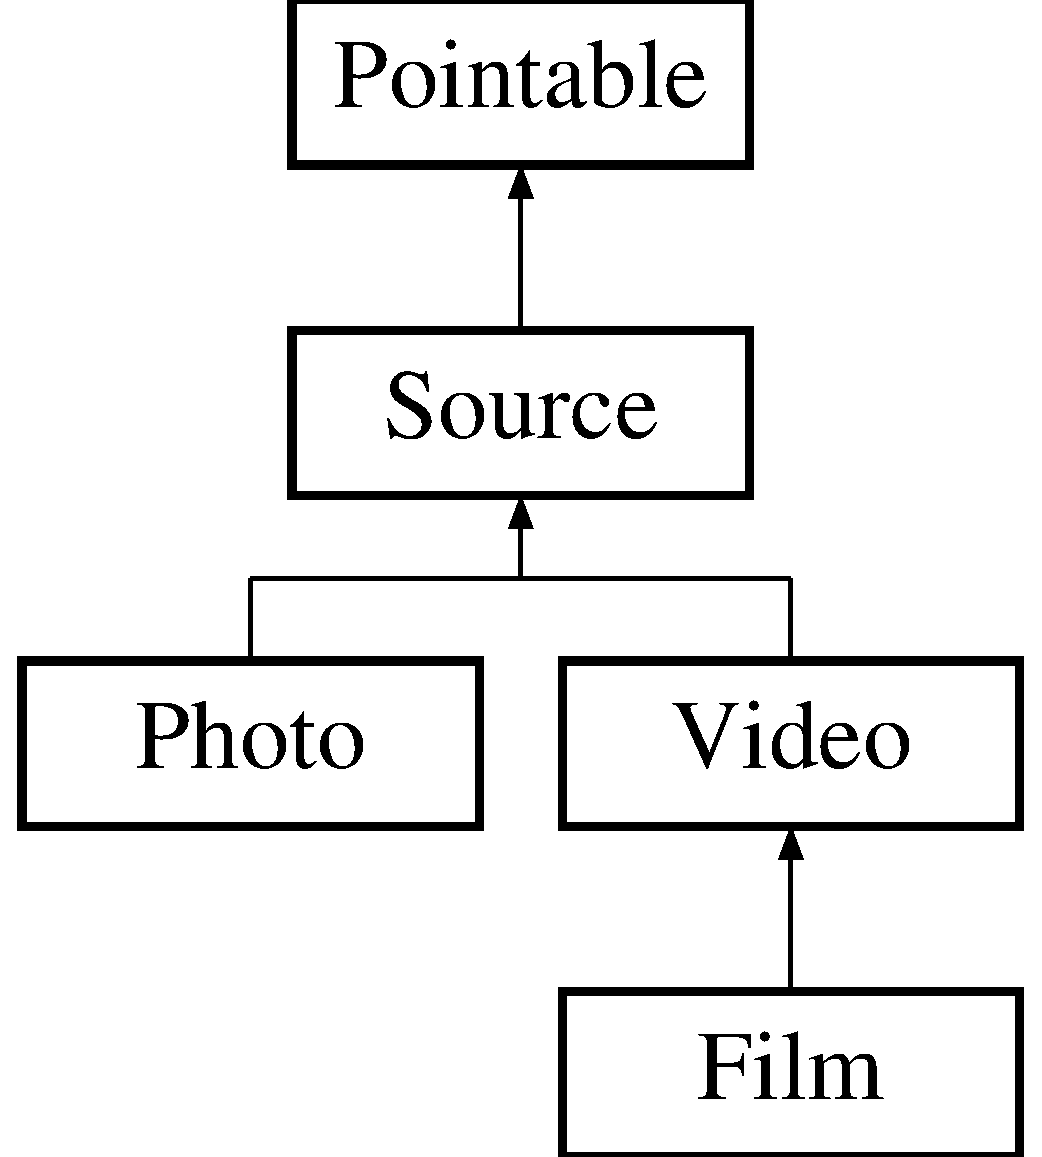
\includegraphics[height=4.000000cm]{classSource}
\end{center}
\end{figure}
\subsection*{Public Member Functions}
\begin{DoxyCompactItemize}
\item 
\hypertarget{classSource_a660c0a4b8b8f8402568bef86f2cb2fbb}{\hyperlink{classSource_a660c0a4b8b8f8402568bef86f2cb2fbb}{Source} ()}\label{classSource_a660c0a4b8b8f8402568bef86f2cb2fbb}

\begin{DoxyCompactList}\small\item\em Constructeur. \end{DoxyCompactList}\item 
\hypertarget{classSource_a446df9431f3636214dea4623cfe31c2b}{{\bfseries Source} (string \-\_\-obj\-Name)}\label{classSource_a446df9431f3636214dea4623cfe31c2b}

\item 
\hypertarget{classSource_ab16c58b57141f64da1fbdc76c70959aa}{{\bfseries Source} (string \-\_\-obj\-Name, string path\-Prefix)}\label{classSource_ab16c58b57141f64da1fbdc76c70959aa}

\item 
\hypertarget{classSource_a6d881583ac7e854493b3bebdeebb0255}{{\bfseries Source} (string \-\_\-obj\-Name, long \-\_\-date, string path\-Prefix)}\label{classSource_a6d881583ac7e854493b3bebdeebb0255}

\item 
\hypertarget{classSource_ac5104a4d66641ae529419b47da4a1473}{virtual \hyperlink{classSource_ac5104a4d66641ae529419b47da4a1473}{$\sim$\-Source} ()}\label{classSource_ac5104a4d66641ae529419b47da4a1473}

\begin{DoxyCompactList}\small\item\em destructeur \end{DoxyCompactList}\item 
\hypertarget{classSource_a5cfde2c99b9dae85f6c6fdd8b4bddb2e}{virtual string \hyperlink{classSource_a5cfde2c99b9dae85f6c6fdd8b4bddb2e}{get\-Obj\-Name} () const }\label{classSource_a5cfde2c99b9dae85f6c6fdd8b4bddb2e}

\begin{DoxyCompactList}\small\item\em retourne le nom de l'objet \end{DoxyCompactList}\item 
\hypertarget{classSource_a51690d970856cc094b271b640692ffef}{virtual long \hyperlink{classSource_a51690d970856cc094b271b640692ffef}{get\-Date} () const }\label{classSource_a51690d970856cc094b271b640692ffef}

\begin{DoxyCompactList}\small\item\em retourne la date d'acquisition de l'objet \end{DoxyCompactList}\item 
\hypertarget{classSource_ad3b0a944c39d7276a777e5bb0b311b87}{virtual string \hyperlink{classSource_ad3b0a944c39d7276a777e5bb0b311b87}{get\-File\-Name} () const }\label{classSource_ad3b0a944c39d7276a777e5bb0b311b87}

\begin{DoxyCompactList}\small\item\em retourne le chemin complet du fichier \end{DoxyCompactList}\item 
\hypertarget{classSource_a156a1f9c3491338d0999b2e9c92877a7}{virtual void \hyperlink{classSource_a156a1f9c3491338d0999b2e9c92877a7}{set\-Obj\-Name} (string \-\_\-obj\-Name)}\label{classSource_a156a1f9c3491338d0999b2e9c92877a7}

\begin{DoxyCompactList}\small\item\em modifie le nom de l'objet \end{DoxyCompactList}\item 
\hypertarget{classSource_a7ff11a007b50f85f26940f9e7feea7c2}{virtual void \hyperlink{classSource_a7ff11a007b50f85f26940f9e7feea7c2}{set\-Date} (long date)}\label{classSource_a7ff11a007b50f85f26940f9e7feea7c2}

\begin{DoxyCompactList}\small\item\em modifie la date d'acquisition de l'objet \end{DoxyCompactList}\item 
\hypertarget{classSource_a96ef6caf2dcf27f6f8b62a128cf912a1}{virtual void \hyperlink{classSource_a96ef6caf2dcf27f6f8b62a128cf912a1}{set\-File\-Name} (string \-\_\-file\-Name)}\label{classSource_a96ef6caf2dcf27f6f8b62a128cf912a1}

\begin{DoxyCompactList}\small\item\em modifie le chemin complet du fichier \end{DoxyCompactList}\item 
\hypertarget{classSource_a4fe532fb822809ff3bd70560a04908bd}{virtual void \hyperlink{classSource_a4fe532fb822809ff3bd70560a04908bd}{print} () const }\label{classSource_a4fe532fb822809ff3bd70560a04908bd}

\begin{DoxyCompactList}\small\item\em affichage \end{DoxyCompactList}\item 
\hypertarget{classSource_aee6e77aa558275f03bb6485d2ed0560f}{virtual std\-::stringstream \& \hyperlink{classSource_aee6e77aa558275f03bb6485d2ed0560f}{print\-To\-Stream} (stringstream \&stream) const }\label{classSource_aee6e77aa558275f03bb6485d2ed0560f}

\begin{DoxyCompactList}\small\item\em ecrit la sortie dans un stringstream \end{DoxyCompactList}\item 
\hypertarget{classSource_a417bae7a27d9a147482df26134400967}{virtual void \hyperlink{classSource_a417bae7a27d9a147482df26134400967}{play} () const =0}\label{classSource_a417bae7a27d9a147482df26134400967}

\begin{DoxyCompactList}\small\item\em play \end{DoxyCompactList}\end{DoxyCompactItemize}
\subsection*{Protected Attributes}
\begin{DoxyCompactItemize}
\item 
\hypertarget{classSource_a920e8bd83e0b0228fe1cb3162f5c1a02}{string {\bfseries obj\-Name}}\label{classSource_a920e8bd83e0b0228fe1cb3162f5c1a02}

\item 
\hypertarget{classSource_a636219480c2ee26eaebadc4f7d08fc68}{long int {\bfseries date}}\label{classSource_a636219480c2ee26eaebadc4f7d08fc68}

\item 
\hypertarget{classSource_aed1da03c1c13ca11fd7bb0405b555923}{string {\bfseries file\-Name}}\label{classSource_aed1da03c1c13ca11fd7bb0405b555923}

\end{DoxyCompactItemize}


\subsection{Detailed Description}
classe de base de multimedia abstraite 

The documentation for this class was generated from the following files\-:\begin{DoxyCompactItemize}
\item 
source.\-h\item 
source.\-cpp\end{DoxyCompactItemize}

\hypertarget{classTCPServer}{\section{T\-C\-P\-Server Class Reference}
\label{classTCPServer}\index{T\-C\-P\-Server@{T\-C\-P\-Server}}
}


{\ttfamily \#include $<$T\-C\-P\-Server.\-h$>$}

\subsection*{Classes}
\begin{DoxyCompactItemize}
\item 
struct \hyperlink{structTCPServer_1_1Hook}{Hook}
\end{DoxyCompactItemize}
\subsection*{Public Member Functions}
\begin{DoxyCompactItemize}
\item 
\hypertarget{classTCPServer_a7a1cd88232db7a3551923ac4fafbad27}{{\bfseries T\-C\-P\-Server} (int buffer\-\_\-size=1000)}\label{classTCPServer_a7a1cd88232db7a3551923ac4fafbad27}

\item 
virtual int \hyperlink{classTCPServer_a1409041961e91f1dbc4933483b4c3b23}{run} (int port)
\end{DoxyCompactItemize}
\subsection*{Protected Member Functions}
\begin{DoxyCompactItemize}
\item 
virtual bool \hyperlink{classTCPServer_a707f8004c0fc8c50aafd12d187b853b9}{process\-Message} (const std\-::string \&message, std\-::string \&response)
\begin{DoxyCompactList}\small\item\em processes a message; the connection will be closed if false is returned. \end{DoxyCompactList}\item 
\hypertarget{classTCPServer_a5d1c3dced9ab7bdc5d5f13866f1eee79}{virtual void \hyperlink{classTCPServer_a5d1c3dced9ab7bdc5d5f13866f1eee79}{read\-Messages} (\hyperlink{classSocket}{Socket} $\ast$)}\label{classTCPServer_a5d1c3dced9ab7bdc5d5f13866f1eee79}

\begin{DoxyCompactList}\small\item\em reads messages from a given socket. \end{DoxyCompactList}\end{DoxyCompactItemize}
\subsection*{Static Protected Member Functions}
\begin{DoxyCompactItemize}
\item 
\hypertarget{classTCPServer_a4b1fcd6fb0425d404f1b07a708c6f0f5}{static void $\ast$ \hyperlink{classTCPServer_a4b1fcd6fb0425d404f1b07a708c6f0f5}{start\-Read\-Message\-Thread} (void $\ast$hook)}\label{classTCPServer_a4b1fcd6fb0425d404f1b07a708c6f0f5}

\begin{DoxyCompactList}\small\item\em starts a thread for reading messages; the argument mus be a \hyperlink{structTCPServer_1_1Hook}{Hook}. \end{DoxyCompactList}\end{DoxyCompactItemize}
\subsection*{Protected Attributes}
\begin{DoxyCompactItemize}
\item 
\hypertarget{classTCPServer_a2399732a7af844b9a314e03a68fd6195}{\hyperlink{classServerSocket}{Server\-Socket} {\bfseries servsock}}\label{classTCPServer_a2399732a7af844b9a314e03a68fd6195}

\item 
\hypertarget{classTCPServer_ab8bc6d00f236389ff0c89a140507f4fa}{std\-::vector$<$ pthread\-\_\-t $>$ {\bfseries threads}}\label{classTCPServer_ab8bc6d00f236389ff0c89a140507f4fa}

\end{DoxyCompactItemize}


\subsection{Detailed Description}
T\-C\-P/\-I\-P command server for remote clients. Commands are executed sequentially (no threads) 

\subsection{Member Function Documentation}
\hypertarget{classTCPServer_a707f8004c0fc8c50aafd12d187b853b9}{\index{T\-C\-P\-Server@{T\-C\-P\-Server}!process\-Message@{process\-Message}}
\index{process\-Message@{process\-Message}!TCPServer@{T\-C\-P\-Server}}
\subsubsection[{process\-Message}]{\setlength{\rightskip}{0pt plus 5cm}bool T\-C\-P\-Server\-::process\-Message (
\begin{DoxyParamCaption}
\item[{const std\-::string \&}]{message, }
\item[{std\-::string \&}]{response}
\end{DoxyParamCaption}
)\hspace{0.3cm}{\ttfamily [protected]}, {\ttfamily [virtual]}}}\label{classTCPServer_a707f8004c0fc8c50aafd12d187b853b9}


processes a message; the connection will be closed if false is returned. 

process message, react to telecommand from Client lister tous les objets

ou recherche un objet et l'afficher au cote client

ou trouver et jouer un objet au cote serveur \hypertarget{classTCPServer_a1409041961e91f1dbc4933483b4c3b23}{\index{T\-C\-P\-Server@{T\-C\-P\-Server}!run@{run}}
\index{run@{run}!TCPServer@{T\-C\-P\-Server}}
\subsubsection[{run}]{\setlength{\rightskip}{0pt plus 5cm}int T\-C\-P\-Server\-::run (
\begin{DoxyParamCaption}
\item[{int}]{port}
\end{DoxyParamCaption}
)\hspace{0.3cm}{\ttfamily [virtual]}}}\label{classTCPServer_a1409041961e91f1dbc4933483b4c3b23}
starts the main loop of the server on this port. returns 0 for normal termination, a value $<$ 0 for an error\-: F\-A\-I\-L\-E\-D = -\/1, U\-N\-K\-N\-O\-W\-N\-\_\-\-H\-O\-S\-T = -\/2, I\-N\-V\-A\-L\-I\-D\-\_\-\-S\-O\-C\-K\-E\-T = -\/3 

The documentation for this class was generated from the following files\-:\begin{DoxyCompactItemize}
\item 
T\-C\-P\-Server.\-h\item 
T\-C\-P\-Server.\-cpp\end{DoxyCompactItemize}

\hypertarget{classVideo}{\section{Video Class Reference}
\label{classVideo}\index{Video@{Video}}
}


The \hyperlink{classVideo}{Video} class heritee de la classe \hyperlink{classSource}{Source}.  




{\ttfamily \#include $<$video.\-h$>$}

Inheritance diagram for Video\-:\begin{figure}[H]
\begin{center}
\leavevmode
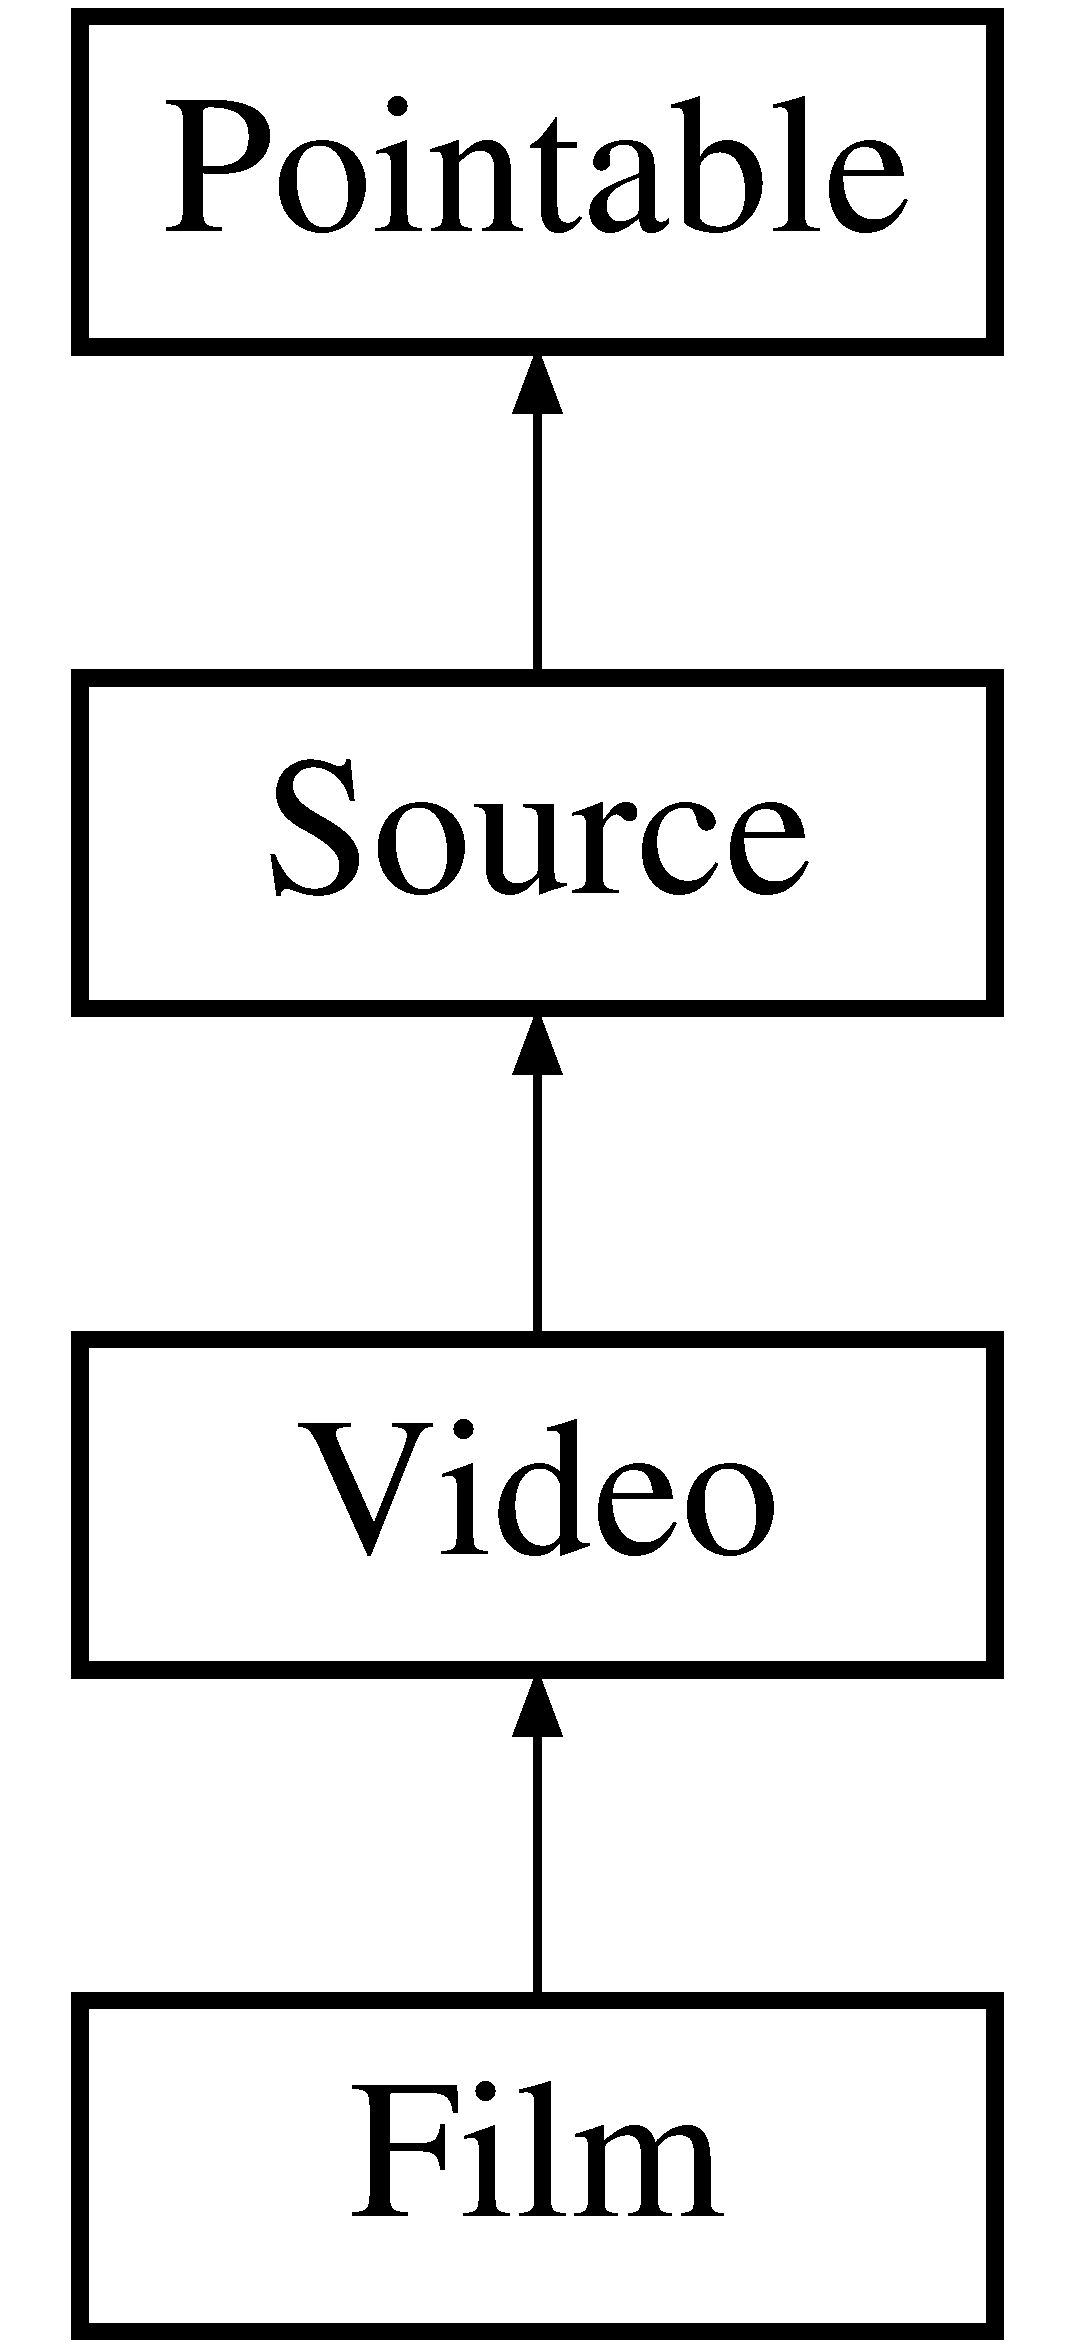
\includegraphics[height=4.000000cm]{classVideo}
\end{center}
\end{figure}
\subsection*{Public Member Functions}
\begin{DoxyCompactItemize}
\item 
\hypertarget{classVideo_ab67336c2c5b6227a9635bc7dcd6af543}{\hyperlink{classVideo_ab67336c2c5b6227a9635bc7dcd6af543}{Video} ()}\label{classVideo_ab67336c2c5b6227a9635bc7dcd6af543}

\begin{DoxyCompactList}\small\item\em constructeur \end{DoxyCompactList}\item 
\hypertarget{classVideo_a186317d34984ad628c3a75c70ba57c64}{{\bfseries Video} (string \-\_\-obj\-Name)}\label{classVideo_a186317d34984ad628c3a75c70ba57c64}

\item 
\hypertarget{classVideo_a721b644bc5cb1b01c65ebe55cb0ce96e}{{\bfseries Video} (string \-\_\-obj\-Name, string path\-Prefix)}\label{classVideo_a721b644bc5cb1b01c65ebe55cb0ce96e}

\item 
\hypertarget{classVideo_aebf7e2a8fa2bbd79335b1cf35925d190}{virtual \hyperlink{classVideo_aebf7e2a8fa2bbd79335b1cf35925d190}{$\sim$\-Video} ()}\label{classVideo_aebf7e2a8fa2bbd79335b1cf35925d190}

\begin{DoxyCompactList}\small\item\em destructeur \end{DoxyCompactList}\item 
virtual int \hyperlink{classVideo_ac8fae47847a7a52762e9b167f52a9bfd}{get\-Duration} () const 
\begin{DoxyCompactList}\small\item\em retourne la duree du video \end{DoxyCompactList}\item 
\hypertarget{classVideo_acceac3b8030a10e7d7fe4778c729abea}{virtual void \hyperlink{classVideo_acceac3b8030a10e7d7fe4778c729abea}{set\-Duration} (int \-\_\-dur)}\label{classVideo_acceac3b8030a10e7d7fe4778c729abea}

\begin{DoxyCompactList}\small\item\em modifie la duree \end{DoxyCompactList}\item 
\hypertarget{classVideo_ab554ec75296a52a815ef1cd0cca4d574}{virtual void \hyperlink{classVideo_ab554ec75296a52a815ef1cd0cca4d574}{print} () const }\label{classVideo_ab554ec75296a52a815ef1cd0cca4d574}

\begin{DoxyCompactList}\small\item\em affichage \end{DoxyCompactList}\item 
\hypertarget{classVideo_a4b4f813aa3c1ab96976c443a897ca6a4}{virtual std\-::stringstream \& \hyperlink{classVideo_a4b4f813aa3c1ab96976c443a897ca6a4}{print\-To\-Stream} (stringstream \&stream) const }\label{classVideo_a4b4f813aa3c1ab96976c443a897ca6a4}

\begin{DoxyCompactList}\small\item\em ecrire la descriptio dans un stringstream \end{DoxyCompactList}\item 
\hypertarget{classVideo_acb8fdb5186d3b35672b9218375cf4f0b}{virtual void \hyperlink{classVideo_acb8fdb5186d3b35672b9218375cf4f0b}{play} () const }\label{classVideo_acb8fdb5186d3b35672b9218375cf4f0b}

\begin{DoxyCompactList}\small\item\em play \end{DoxyCompactList}\end{DoxyCompactItemize}
\subsection*{Protected Attributes}
\begin{DoxyCompactItemize}
\item 
\hypertarget{classVideo_a8534071e7e759e39c42fa9a51ae620eb}{int {\bfseries duration}}\label{classVideo_a8534071e7e759e39c42fa9a51ae620eb}

\end{DoxyCompactItemize}


\subsection{Detailed Description}
The \hyperlink{classVideo}{Video} class heritee de la classe \hyperlink{classSource}{Source}. 

\subsection{Member Function Documentation}
\hypertarget{classVideo_ac8fae47847a7a52762e9b167f52a9bfd}{\index{Video@{Video}!get\-Duration@{get\-Duration}}
\index{get\-Duration@{get\-Duration}!Video@{Video}}
\subsubsection[{get\-Duration}]{\setlength{\rightskip}{0pt plus 5cm}int Video\-::get\-Duration (
\begin{DoxyParamCaption}
{}
\end{DoxyParamCaption}
) const\hspace{0.3cm}{\ttfamily [virtual]}}}\label{classVideo_ac8fae47847a7a52762e9b167f52a9bfd}


retourne la duree du video 

retourne la duree 

The documentation for this class was generated from the following files\-:\begin{DoxyCompactItemize}
\item 
video.\-h\item 
video.\-cpp\end{DoxyCompactItemize}

%--- End generated contents ---

% Index
\newpage
\phantomsection
\addcontentsline{toc}{chapter}{Index}
\printindex

\end{document}
